%% =====================================================================
%% StoHyMoLAP -- Ramis basin manuscript (REVISED VERSION WITH CITATIONS)
%% Elsevier CAS single-column class (cas-sc.cls).
%%
%% REVISION NOTES:
%%  - Introduction, Methods, Discussion rewritten with targeted citations
%%    from the provided bibliography annotation package.
%%  - Citation style: \citep{} for parenthetical, \citet{} for narrative.
%%  - Placeholders marked %% [FILL] as before.
%% =====================================================================
\documentclass[a4paper,fleqn]{cas-sc}

\usepackage[authoryear,longnamesfirst]{natbib}
\usepackage{amsmath,amssymb}
\usepackage{booktabs}
\usepackage{graphicx}
\usepackage{tabularx}
\usepackage{threeparttable}
\usepackage{multirow}
\usepackage{siunitx}
\usepackage{xspace}
\usepackage{url}
\usepackage{float}
\usepackage{enumitem}

\begin{document}
\let\WriteBookmarks\relax
\def\floatpagepagefraction{1}
\def\textpagefraction{.001}

\shorttitle{Stochastic physical-ensemble quantiles for streamflow hybridization}
\shortauthors{Zevallos}

\title[mode = title]{Stochastic Physical-Ensemble Quantiles Improve Hybrid
Machine-Learning Simulation of Daily Streamflow in the High-Andean Ramis Basin}

% First author
\author[1]{Jose Zevallos}[orcid=0000-0002-6023-8665]
\cormark[1]
\ead{20240318@lamolina.edu.pe}
\credit{Conceptualization of this study, Methodology, Software, Writing -- original draft}

% Address/affiliation
\affiliation[1]{organization={Centro de Investigaci\'{o}n y Tecnolog\'{i}a del Agua (CITA), Universidad de Ingenier\'{i}a y Tecnolog\'{i}a (UTEC)},
                addressline={Jr. Medrano Silva 165, Barranco},
                city={Lima},
                postcode={15063},
                state={Lima},
                country={Peru}}

\cortext[1]{Corresponding author.}

%% =====================================================================
%% ABSTRACT
%% =====================================================================
\begin{abstract}
Hybrid hydrological modelling combines process-based structure with the
predictive flexibility of machine learning (ML), but often leaves unclear
which component drives improved streamflow prediction. We present
StoHyMoLAP, a reproducible and audit-controlled framework for daily
streamflow simulation in the high-Andean Ramis basin, within the Lake
Titicaca system of southern Peru. The framework couples a lumped RAMIS
rainfall--runoff core, an optional linear baseflow reservoir,
L\'{e}vy-type ($\alpha$-stable) stochastic perturbations, Monte Carlo
physical ensembles, and ML emulators trained from observed forcings or
from stochastic-ensemble descriptors. Nine experiments (E0--E8) were
evaluated over a common validation window from 8~January~2009 to
31~December~2020 ($n=4367$ daily samples), with temporal-leakage and
backend audits embedded in the evidence chain.

Quantile descriptors from the stochastic physical ensemble provided the
largest robust gain. The gradient-boosting quantile hybrid reached
NSE\,=\,0.740 and KGE\,=\,0.810, improving NSE by 0.311 relative to the
complete stochastic physical model and by 0.165 relative to the pure ML
baseline. Replacing ensemble-mean features with ensemble quantiles
alone added 0.114 NSE, showing that distributional physical descriptors
contain information not captured by a single mean trajectory. The
baseflow reservoir modestly improved the deterministic physical
baseline, whereas direct L\'{e}vy perturbations produced inconsistent
point-prediction gains. The stochastic physical bands were strongly
underdispersive (PICP\,=\,0.004 against a nominal 0.95 target), so the
ensemble is more useful as ML features than as calibrated predictive
uncertainty. The numerically best run (NSE\,=\,0.849, KGE\,=\,0.899,
RMSE\,=\,0.210~m$^3$\,s$^{-1}$) was labelled as GRU but executed as a
fallback multilayer perceptron on flattened sequences; it is not
evidence of recurrent-network superiority. These findings support
stochastic physical--ML hybridization while showing that uncertainty
calibration, low-flow correction and backend-aware reporting remain
essential for defensible hydrological modelling.
\end{abstract}

\begin{highlights}
\item Ensemble quantiles were the dominant driver of hybrid streamflow skill.
\item The quantile hybrid improved NSE by 0.311 over stochastic RAMIS.
\item L\'{e}vy perturbations informed ML features but underdispersed intervals.
\item Backend and leakage audits constrained claims for GRU-labelled runs.
\item The ablation separated memory, stochasticity, ML and descriptors.
\end{highlights}

\begin{keywords}
Daily streamflow simulation \sep Stochastic hydrological modelling \sep
Physical--machine learning hybridization \sep Ensemble quantiles \sep
Uncertainty diagnostics \sep High-Andean basin
\end{keywords}

\maketitle

%% =====================================================================
%% 1. INTRODUCTION
%% =====================================================================
\section{Introduction}\label{sec:introduction}

Reliable daily streamflow simulation remains a central problem in
surface-water hydrology, particularly in basins where observations are
sparse, hydroclimatic variability is strong and operational decisions
must still be supported by defensible discharge estimates
\citep{razavi2013streamflow,guo2021regionalization}. These conditions
are characteristic of many high-elevation Andean catchments. In the
Peruvian Altiplano, precipitation is strongly seasonal, monitoring
networks are sparse relative to the spatial heterogeneity of rainfall,
and discharge dynamics are shaped by the alternation between sharp
wet-season runoff response and sustained dry-season low flows
\citep{condom2004transient,zubieta2018hydrological,lima2025modeling}.
Such settings expose a persistent limitation of classical
rainfall--runoff modelling: even when a conceptual model captures the
main water-balance controls, simplified storage structures, uncertain
parameters and imperfect meteorological inputs can lead to structural
errors that become particularly visible under low-flow, flashy or
climatically contrasting conditions
\citep{van2013influence,nauditt2017conceptual,ragettli2014evaluation}.

Machine-learning (ML) models offer a complementary route because they
can learn nonlinear rainfall--runoff relations directly from data. Large
sample studies have shown that recurrent and other data-driven models
can match or outperform lumped conceptual models in daily streamflow
prediction, including in regional and basin-scale benchmarks
\citep{kratzert2019towards,lees2021benchmarking,arsenault2022continuous}.
However, predictive skill alone does not eliminate hydrological risk.
Purely data-driven models may be sensitive to distributional shifts,
training-period representativeness, extrapolation to extremes and the
absence of explicit physical constraints
\citep{frame2021deep,zhong2023developing}. In data-scarce basins, their
performance also depends strongly on whether antecedent hydrological
state information is available, because rainfall inputs alone may be
insufficient to represent catchment memory
\citep{adnan2021comparison,okkan2021embedding}. The practical question
is therefore not whether process-based or ML models are universally
superior, but how physical structure and empirical flexibility can be
combined without obscuring the source of any improvement.

Hybrid physical--ML modelling addresses this question by using process
simulations, physically derived states or synthetic physically
consistent samples as inputs to an empirical emulator. This strategy has
improved runoff simulation in several configurations, including
conceptual-model correction, nested hybrid rainfall--runoff modelling,
physics-guided deep learning and process-driven deep learning
\citep{mekonnen2015hybrid,mohammadi2022ihacres,okkan2021embedding,yang2020physical,xie2021physics,li2024process,zhu2025hybrid}.
Most of these studies, however, pass forward a deterministic physical
trajectory. That design preserves part of the process information but
collapses the conditional distribution of the simulated response into a
single value. For stochastic rainfall--runoff transformation, this is a
strong simplification: uncertainty in precipitation, model structure and
hydrological memory propagates nonlinearly into discharge and can alter
both peak timing and magnitude
\citep{gabellani2007propagation,hong2006uncertainty}. It also limits the
ability of the hybrid model to exploit distributional descriptors such
as ensemble quantiles, which are closely related to hydrological
signatures and to probabilistic forecasting diagnostics
\citep{guo2021regionalization,papacharalampous2022review}.

A recent stochastic hybridization study by
\citet{houenafa2025hybridization} showed that mean and quantile
descriptors of a L\'{e}vy-driven stochastic HyMoLAP discharge ensemble
can improve ML-based rainfall--runoff prediction. This result is
important because it moves physical--ML hybridization from deterministic
state correction toward distribution-aware physical descriptors. Yet it
also leaves three issues unresolved. First, the gain from the hybrid
pipeline may come from several components---hydrological memory,
stochastic perturbations, the ML correction itself or the use of
quantile rather than mean ensemble descriptors---and these effects are
not identifiable from a single best-model comparison. Second, a
stochastic ensemble that improves point prediction is not necessarily a
calibrated predictive interval; coverage, sharpness and interval scores
must be evaluated separately. Third, reproducibility claims require that
reported model labels match the backend that actually produced the
results, especially when deep-learning architectures have software
fallbacks or implementation contingencies.

This study addresses these gaps through StoHyMoLAP, an audited
stochastic physical--ML framework for daily streamflow simulation in the
high-Andean Ramis basin, the principal tributary of Lake Titicaca. The
framework couples a lumped RAMIS rainfall--runoff core, an optional
linear baseflow reservoir, L\'{e}vy-type stochastic perturbations,
Monte Carlo physical ensembles and ML emulators trained either from
observed forcings or from physical-ensemble descriptors. The purpose is
not to introduce another best-performing hybrid model, but to decompose
which components are responsible for performance gains. Nine controlled
experiments (E0--E8; Table~\ref{tab:experiment-matrix}) are therefore
evaluated over a common validation window using a single workflow
(Fig.~\ref{fig:method-workflow}). The ablation design isolates the
incremental roles of baseflow memory, stochastic forcing, ML correction
and descriptor choice.

The manuscript makes four specific contributions. First, it transfers
stochastic physical--ML quantile hybridization to a high-Andean,
strongly seasonal and data-scarce Altiplano basin, providing a contrast
to previous applications outside this hydroclimatic setting. Second, it
shows whether ensemble mean or ensemble quantiles carry the more useful
physical information for ML correction. Third, it evaluates the same
stochastic ensemble both as a source of predictive features and as a
candidate uncertainty band through PICP, PINAW and Winkler diagnostics.
Fourth, it embeds temporal-leakage and backend audits into the evidence
chain, following the broader call for transparent and reproducible
hydrological modelling \citep{hall2021hydrologist}. A key audit finding
is stated explicitly: the experiments labelled as GRU in the current
run were executed with a fallback multilayer perceptron on flattened
sequences, not with a true recurrent backend. They are therefore
interpreted as GRU-labelled sequential hybrids under fallback execution,
not as evidence of recurrent-network superiority
\citep{kratzert2018rainfall}.

%% =====================================================================
%% 2. MATERIALS AND METHODS
%% =====================================================================
\section{Materials and methods}\label{sec:methods}

\subsection{Study area}\label{subsec:study-area}

The Ramis River basin is located in the high-Andean Altiplano of
southern Peru and drains towards Lake Titicaca. The basin is therefore
part of a closed lacustrine system in which river inflow, precipitation
and evaporation exert strong control on lake-level variability
\citep{cross2001late,condom2004transient,lima2025modeling}. Previous
regional studies show that the hydrology of the Titicaca system is
controlled mainly by rainfall and evapotranspiration variability,
whereas snowmelt, ice melt and net irrigation withdrawals have a
secondary role at the lake-basin scale \citep{lima2025modeling}. This
regional behaviour makes the Ramis basin a relevant test case for a
rainfall--runoff framework designed to combine process-based memory,
stochastic forcing and machine-learning correction.

The basin is characterized by high elevation, sparse hydroclimatic
monitoring and a strongly seasonal precipitation regime. Rainfall is
concentrated during the austral summer wet season, while the dry season
is associated with prolonged recession and low-flow persistence
\citep{condom2004transient,nauditt2017conceptual,lima2025modeling}.
Such hydroclimatic asymmetry is challenging for lumped conceptual
models because a single storage response may be unable to represent both
wet-season peaks and dry-season baseflow. It is also challenging for
purely data-driven models, which may learn strong seasonal correlations
without representing the storage mechanisms that maintain discharge
between rainfall events \citep{van2013influence,lees2021benchmarking}.
Daily discharge observations used in this study correspond to the
Puente Ramis gauging station operated by SENAMHI-Peru.

%% [AUTHOR ACTION BEFORE SUBMISSION]
%% Insert the official gauged drainage area, station coordinates, gauge
%% elevation and complete record period from SENAMHI/ANA metadata. These
%% details were not included in the evidence package used for this phase
%% and should not be inferred.

\subsection{Hydro-meteorological data and temporal protocol}
\label{subsec:data-protocol}

The modelling unit is a daily hydro-meteorological record composed of
precipitation ($P_t$), minimum and maximum temperature
($T_{\min,t}$ and $T_{\max,t}$), potential evapotranspiration
($PET_t$) and observed streamflow ($Q^{obs}_t$). The rainfall--runoff
core uses an effective precipitation input defined as
\begin{equation}
P^{eff}_t = \max(P_t - PET_t,\;0),
\label{eq:peff}
\end{equation}
which provides a non-negative approximation of the water available for
runoff generation after atmospheric demand has been accounted for.

All experiments follow the same chronological split. Model calibration
and ML training use data from 8~September~1991 to 31~December~2008,
whereas validation uses data from 8~January~2009 to 31~December~2020.
The final leaderboard is computed over the common validation
intersection of all experiments, comprising $n=4367$ daily samples. This
common-window design prevents unequal evaluation support across
physical, ML and hybrid configurations and is especially important for
experiments that require lagged predictors or sequence construction.

Temporal leakage was controlled at four levels. First, lagged predictors
were constructed only from present or past information. Second,
sequence samples were generated independently within the training and
validation partitions. Third, scalers and transformations used by ML
models were fitted exclusively on training data and then applied to
validation data. Fourth, flow-regime thresholds used for diagnostic
stratification were estimated from training observations only. These
controls follow the broader hydrological ML recommendation that model
selection and preprocessing must preserve temporal ordering
\citep{arsenault2022continuous,chen2013finding}. The corresponding
audit status is reported in Table~\ref{tab:reproducibility}.

\subsection{Lumped rainfall--runoff core}\label{subsec:physical-core}

Although the implementation workflow occasionally uses the term
``hydrodynamic'', the model evaluated here is a lumped stochastic
rainfall--runoff simulator, not a spatially distributed hydraulic or
hydrodynamic solver. The process-based component is therefore described
as a catchment-scale discharge-dynamics model. Its fast-flow state is
represented by the recurrence
\begin{equation}
x_t = \left(1 - \frac{\mu}{\lambda}\right)x_{t-1} + P^{eff}_t,
\label{eq:ramis-state}
\end{equation}
where $\mu>0$ and $\lambda>0$ regulate catchment memory and recession
stability. The parameter constraint $0<\mu/\lambda<1$ ensures a stable,
non-oscillatory memory factor.

The fast-flow discharge component is updated as
\begin{equation}
Q^{fast}_t = Q^{fast}_{t-1}
  - \frac{\mu}{\lambda}\,Q_0
    \left(\frac{\max(Q^{fast}_{t-1},0)}{Q_0}\right)^{2\mu-1}
  + \frac{\alpha_A}{\lambda}\,x_{t-1}
  + \sigma\,Q^{fast}_{t-1}\,\Delta L_t,
\label{eq:ramis-fast}
\end{equation}
where $Q_0$ is a reference discharge, $\alpha_A$ is an empirical
conversion factor, $\sigma$ controls stochastic amplitude and
$\Delta L_t$ is a stochastic increment. In deterministic experiments,
the stochastic term is inactive. Negative simulated discharge is clipped
to zero when non-negative physical post-processing is enabled.

The recurrence in Eqs.~\ref{eq:ramis-state}--\ref{eq:ramis-fast}
represents catchment-scale nonlinearity through aggregated storage
behaviour. This interpretation is consistent with recession analyses in
which nonlinear catchment response can emerge from heterogeneous linear
storage elements rather than from a single local nonlinear mechanism
\citep{harman2009power}. In this setting, the parameter $\mu$ acts as a
shape parameter controlling the effective recession behaviour of the
lumped storage system.

\subsection{Linear baseflow reservoir}\label{subsec:baseflow}

An optional linear reservoir is used to represent hydrological memory
beyond the fast-flow recurrence. This addition is motivated by previous
work in the Titicaca region showing that groundwater storage fluxes are
important for explaining seasonal runoff persistence and dry-season
baseflow \citep{nauditt2017conceptual}. The reservoir also provides a
controlled way to test whether adding a simple memory component improves
simulation skill before introducing stochastic perturbations or ML
correction.

Recharge to the baseflow store is proportional to effective
precipitation:
\begin{equation}
R_t = c_r\,\alpha_A\,P^{eff}_t,
\label{eq:recharge}
\end{equation}
where $c_r\in[0,1]$ is the recharge coefficient. Storage and baseflow
discharge then evolve as
\begin{align}
S_{b,t+1} &= \max\!\left(0,\;S_{b,t} + R_t - k_b S_{b,t}\right),
\label{eq:storage}\\
Q^{base}_t &= k_b\,S_{b,t},
\label{eq:qbase}
\end{align}
where $k_b\in[0.001,0.5]$ is the linear recession coefficient. The
total process-based discharge is
\begin{equation}
Q^{phys}_t = \max\!\left(Q^{fast}_t + Q^{base}_t,\;0\right).
\label{eq:qtotal}
\end{equation}
The baseflow component is activated in E1, E3 and all hybrid
configurations. Its isolated contribution is evaluated through the
E1--E0 and E3--E2 ablation contrasts.

\subsection{L\'{e}vy perturbations and Monte Carlo physical ensembles}
\label{subsec:levy}

Stochastic physical experiments inject $\alpha$-stable L\'{e}vy-type
increments into Eq.~\ref{eq:ramis-fast}. The perturbation is governed
by stability, skewness, location and scale parameters. Heavy-tailed
increments are used to represent episodic deviations from the smooth
lumped response, which is relevant in a highly seasonal basin where
rainfall inputs and streamflow errors are not expected to be Gaussian.
This design is consistent with hydrological ensemble studies showing
that uncertainty is not limited to the mean response but also involves
dispersion, asymmetry and tail behaviour
\citep{hong2006uncertainty,gabellani2007propagation,abaza2017incidence}.

For each calibrated stochastic configuration, a Monte Carlo ensemble of
$N$ trajectories is generated. At each day, the ensemble is summarized
by central-tendency, dispersion and quantile descriptors. The quantile
set used in the hybrid experiments is
\begin{equation}
\{q_{0.01},\;q_{0.05},\;q_{0.25},\;q_{0.50},\;q_{0.75},
  \;q_{0.95},\;q_{0.99}\},
\label{eq:quantiles}
\end{equation}
together with spread measures such as $q_{0.95}-q_{0.05}$ and
$q_{0.75}-q_{0.25}$. Quantile representations are robust summaries of
non-Gaussian and fat-tailed distributions, and therefore provide a
natural way to pass distributional information from a stochastic
physical ensemble to an ML emulator \citep{swiderski2016aggregation}.
In this study, the same ensemble is evaluated in two roles: as a direct
stochastic physical predictor in E2 and E3, and as a source of
physically informed ML features in E5--E8.

\subsection{Machine-learning emulators and feature sets}
\label{subsec:emulator}

The ML component maps a feature vector $\mathbf{z}_t$ to daily simulated
discharge,
\begin{equation}
\hat{Q}_t = f_\theta(\mathbf{z}_t),
\label{eq:emulator}
\end{equation}
followed by non-negative clipping,
\begin{equation}
Q^{sim}_t = \max(\hat{Q}_t,\;0).
\label{eq:ml-clipping}
\end{equation}
This post-processing step ensures physically admissible discharge
predictions while preserving the fitted ML response over positive
flows.

Three feature families are compared. The pure ML baseline (E4) uses
observed hydro-meteorological forcings and non-negative lags, including
lagged runoff information where allowed by the temporal protocol.
Including antecedent runoff is hydrologically meaningful because it
acts as a proxy for catchment storage and has been shown to improve
rainfall--runoff ML models relative to meteorological predictors alone
\citep{adnan2021comparison}. Mean-based hybrids (E5 and E7) use the
mean trajectory of the stochastic physical ensemble. Quantile-based
hybrids (E6 and E8) use the ensemble quantiles and spread descriptors
listed in Eq.~\ref{eq:quantiles}. This design tests whether the ML
emulator benefits primarily from a corrected central physical trajectory
or from richer distributional descriptors of the physical ensemble.

The tabular emulator is labelled as XGB in the experiment names. In the
current evidence package, however, the actual backend was
\texttt{HistGradientBoostingRegressor} from scikit-learn, reported in
the audit tables as \texttt{sklearn\_hgb}. The corresponding results
are therefore interpreted as gradient-boosted tree hybrids rather than
as package-specific evidence for \texttt{xgboost}. Hyperparameter search
used temporally ordered cross-validation, avoiding random shuffling of
time steps during model selection.

The sequential emulator is labelled as GRU in the experiment names and
is designed to use recurrent layers when a supported backend is
available. In the present execution, the recurrent backend was not
available; the implementation flattened each input sequence and trained
a multilayer perceptron instead. Consequently, E7 and E8 are retained in
the experimental matrix because they evaluate sequentially constructed
features, but they are interpreted throughout the manuscript as
GRU-labelled fallback-MLP runs, not as evidence of true recurrent GRU
superiority \citep{kratzert2018rainfall,kratzert2019towards}.

\subsection{Calibration objective}\label{subsec:calibration}

The process-based and stochastic configurations are calibrated with a
scalar objective that combines efficiency, distributional agreement,
bias and interval coverage:
\begin{equation}
J = \frac{w_{NSE}(1-NSE) + w_{KGE}(1-KGE)
  + w_{PBIAS}\left|\frac{PBIAS}{100}\right|
  + w_{cov}|c^*-PICP|}{w_{active}},
\label{eq:objective}
\end{equation}
where $c^*=0.95$ is the nominal coverage target and $w_{active}$ is the
sum of the active weights. The default weights are $w_{NSE}=0.40$,
$w_{KGE}=0.30$, $w_{PBIAS}=0.15$ and $w_{cov}=0.15$. When a model does
not produce prediction intervals, the coverage term is omitted and the
remaining weights are renormalized.

The composite objective is used because no single deterministic metric
fully describes hydrological model performance, particularly when both
high-flow peaks and low-flow persistence are relevant
\citep{pushpalatha2012review}. The coverage term is included to avoid
selecting stochastic configurations that are sharp but severely
underdispersive, a common limitation in hydrological ensemble
prediction \citep{franz2011evaluating,abaza2017incidence}.

\subsection{Experimental matrix and ablation design}\label{subsec:matrix}

The experimental matrix was designed to isolate the contribution of each
modelling component under a common validation window. E0 and E1 compare
the deterministic RAMIS core without and with the baseflow reservoir.
E2 and E3 add L\'{e}vy stochasticity without and with baseflow. E4 is a
pure ML baseline trained only from observed predictors. E5 and E6 are
gradient-boosting hybrids using, respectively, ensemble-mean and
ensemble-quantile physical descriptors. E7 and E8 use the same mean and
quantile feature families in a sequential-feature setting, but with the
fallback MLP backend described above.

\begin{table*}[t]
\caption{Controlled experimental matrix. Backend entries report the
actual backend used in the current evidence package.}
\label{tab:experiment-matrix}
\centering
\small
\begin{tabular*}{\textwidth}{@{\extracolsep{\fill}}lllllll@{}}
\toprule
Experiment & Family & L\'{e}vy & Baseflow & Emulator & Features
  & Backend used \\
\midrule
E0\_RAMIS\_DET\_NOBF   & physical RAMIS & no  & no  & none
  & physical only & physical \\
E1\_RAMIS\_DET\_BF     & physical RAMIS & no  & yes & none
  & physical only & physical \\
E2\_RAMIS\_LEVY\_NOBF  & RAMIS--L\'{e}vy & yes & no  & none
  & physical only & physical \\
E3\_RAMIS\_LEVY\_BF    & RAMIS--L\'{e}vy & yes & yes & none
  & physical only & physical \\
E4\_ML\_PURE\_XGB      & pure ML        & no  & no  & XGB-labelled
  & observed forcings & sklearn\_hgb \\
E5\_HYB\_XGB\_MEAN     & hybrid         & yes & yes & XGB-labelled
  & ensemble mean & sklearn\_hgb \\
E6\_HYB\_XGB\_QUANTILES & hybrid        & yes & yes & XGB-labelled
  & ensemble quantiles & sklearn\_hgb \\
E7\_HYB\_GRU\_MEAN     & sequential hybrid & yes & yes & GRU-labelled
  & mean sequence & fallback MLP \\
E8\_HYB\_GRU\_QUANTILES & sequential hybrid & yes & yes & GRU-labelled
  & quantile sequence & fallback MLP \\
\bottomrule
\end{tabular*}
\end{table*}

This matrix supports five planned contrasts: the effect of baseflow
(E1--E0 and E3--E2), the direct effect of stochastic perturbations under
baseflow (E3--E1), the effect of pure ML correction relative to the full
stochastic physical model (E4--E3), the effect of hybridization
(E5--E3 and E6--E3), and the value of quantile descriptors relative to
mean descriptors (E6--E5 and E8--E7). The same validation samples are
used in every contrast.

\subsection{Relation to prior stochastic physical--ML hybridization}
\label{subsec:relation}

The idea of feeding descriptors from a stochastic physical ensemble into
an ML emulator is closely related to the hybridization strategy of
\citet{houenafa2025hybridization}. The present study is framed as an
ablation and audit extension of that idea. Rather than reporting only
the best hybrid configuration, it decomposes the pipeline into physical
memory, stochastic perturbation, ML correction and descriptor choice. It
also evaluates whether the same ensemble that improves ML features can
serve as a calibrated predictive uncertainty band. This distinction is
important because physically plausible ensemble spread does not
necessarily imply reliable probabilistic coverage
\citep{atger1999skill,franz2011evaluating,papacharalampous2022review}.

\subsection{Evaluation metrics and audit protocol}\label{subsec:evaluation}

Point-prediction performance is evaluated with Nash--Sutcliffe
efficiency (NSE), Kling--Gupta efficiency (KGE), root mean squared error
(RMSE), mean absolute error (MAE), percent bias (PBIAS) and the
coefficient of determination ($R^2$). Regime-specific metrics are
computed for low, mid and high flows using thresholds estimated from
training observations only. Low-flow NSE is interpreted cautiously
because efficiency scores based on squared error are sensitive to low
observed variance and can penalize dry-season errors in ways that are
not proportional to their hydrological relevance
\citep{pushpalatha2012review}.

Stochastic reference bands are evaluated using prediction interval
coverage probability (PICP), prediction interval normalized average
width (PINAW), mean prediction interval width (MPIW) and Winkler score.
The intended behaviour is high coverage with the narrowest possible
intervals, but sharpness is not interpreted as skill when coverage is
far below the nominal level \citep{franz2011evaluating,abaza2017incidence,papacharalampous2022review}.
The final audit checks chronological split integrity, feature
construction, target leakage, backend metadata, common-window
consistency and non-negative post-processing. The audit results are
reported in Table~\ref{tab:reproducibility}.

\begin{figure*}[t]
\centering
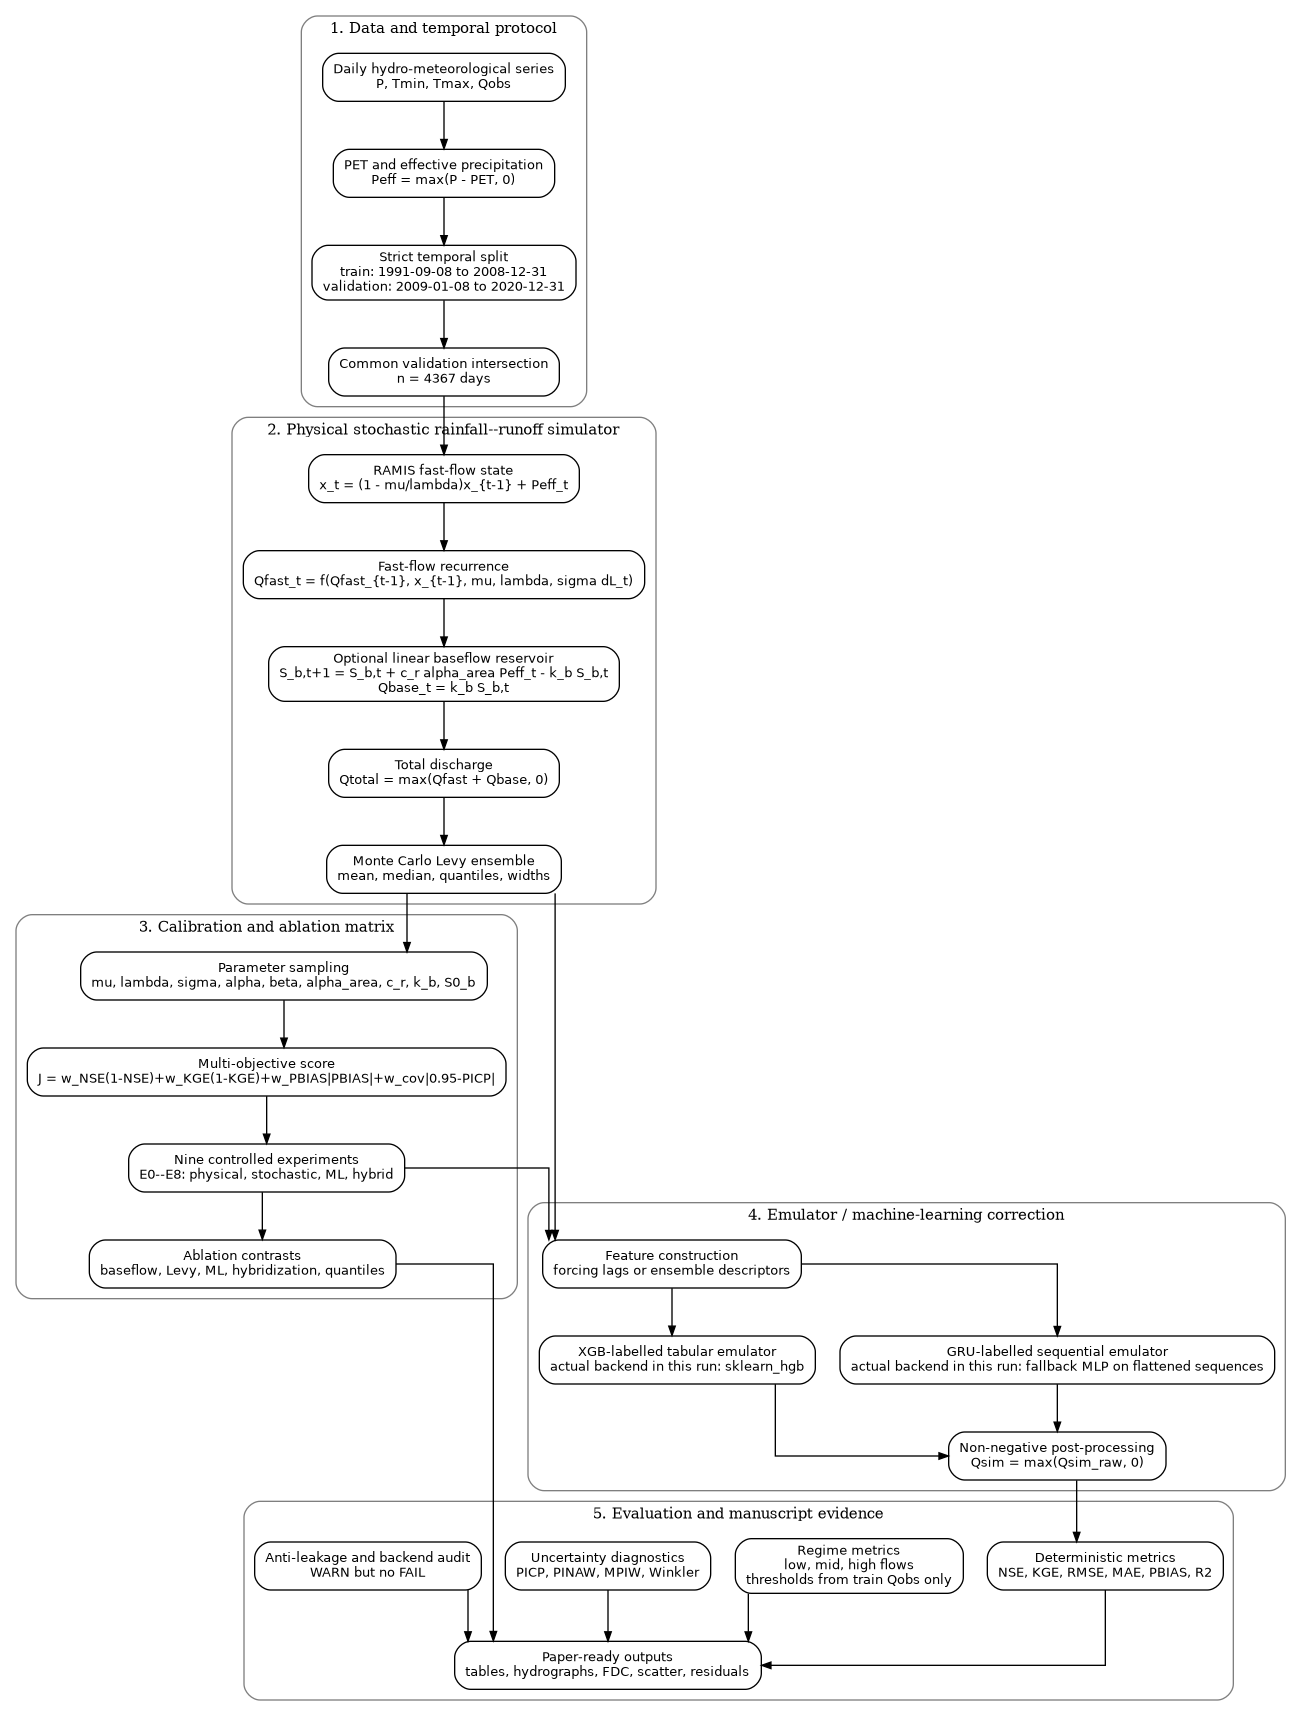
\includegraphics[width=0.96\textwidth]{figures/method_workflow.png}
\caption{StoHyMoLAP workflow from daily hydro-meteorological data to
lumped physical simulation, L\'{e}vy-type stochastic ensemble
generation, ensemble-descriptor construction, ML emulation, ablation
comparison and audit-controlled manuscript evidence.}
\label{fig:method-workflow}
\end{figure*}

%% =====================================================================
%% 3. RESULTS
%% =====================================================================
\section{Results}\label{sec:results}

\subsection{Common-window ranking}\label{subsec:ranking-results}

All experiments were evaluated on the same validation window defined in
Section~\ref{subsec:data-protocol}. Table~\ref{tab:ranking} and
Fig.~\ref{fig:metric-ranking} show a clear separation between the
physical-only baselines, the pure ML baseline and the hybrid
configurations. The deterministic and stochastic physical baselines
(E0--E3) clustered within a narrow NSE range of 0.414--0.438, whereas
the pure forcing-based ML model (E4) reached NSE\,=\,0.575. All hybrid
models exceeded E4 in NSE, indicating that the stochastic physical
ensemble supplied additional predictive information beyond the observed
forcing variables alone.

The strongest \emph{backend-consistent} configuration was
E6\_HYB\_XGB\_QUANTILES, which achieved NSE\,=\,0.740,
KGE\,=\,0.810, RMSE\,=\,0.275~m$^3$\,s$^{-1}$,
MAE\,=\,0.162~m$^3$\,s$^{-1}$ and PBIAS\,=\,0.927\%. This run is the
main evidence for the proposed quantile-based stochastic physical--ML
hybridization because its manuscript label and executed backend are
consistent. The numerically best run was E8\_HYB\_GRU\_QUANTILES
(NSE\,=\,0.849, KGE\,=\,0.899 and RMSE\,=\,0.210~m$^3$\,s$^{-1}$),
but it is interpreted separately because the audit showed that it ran
as a fallback multilayer perceptron on flattened sequences rather than
as a recurrent GRU. The ranking is therefore reported in two layers:
E8 is the best numerical configuration, whereas E6 is the strongest
robust configuration for defensible process-based interpretation.

\begin{table*}[t]
\caption{Final common-window ranking. Metrics are computed on 4367
validation samples from 8 January 2009 to 31 December 2020.}
\label{tab:ranking}
\centering
\small
\begin{tabular*}{\textwidth}{@{\extracolsep{\fill}}rlllllll@{}}
\toprule
Rank & Experiment & NSE & KGE & RMSE & MAE & PBIAS & Backend \\
\midrule
1 & E8\_HYB\_GRU\_QUANTILES   & 0.849 & 0.899 & 0.210 & 0.124
  & 1.579 & fallback\_mlp\_on\_flattened\_sequences \\
2 & E6\_HYB\_XGB\_QUANTILES   & 0.740 & 0.810 & 0.275 & 0.162
  & 0.927 & sklearn\_hgb \\
3 & E7\_HYB\_GRU\_MEAN        & 0.686 & 0.789 & 0.302 & 0.192
  & 1.644 & fallback\_mlp\_on\_flattened\_sequences \\
4 & E5\_HYB\_XGB\_MEAN        & 0.626 & 0.715 & 0.330 & 0.210
  & 2.007 & sklearn\_hgb \\
5 & E4\_ML\_PURE\_XGB         & 0.575 & 0.661 & 0.352 & 0.223
  & 0.742 & sklearn\_hgb \\
6 & E1\_RAMIS\_DET\_BF        & 0.438 & 0.714 & 0.405 & 0.248
  & 0.860 & physical \\
7 & E3\_RAMIS\_LEVY\_BF       & 0.429 & 0.725 & 0.408 & 0.255
  & -1.218 & physical \\
8 & E2\_RAMIS\_LEVY\_NOBF     & 0.427 & 0.717 & 0.409 & 0.268
  & -7.551 & physical \\
9 & E0\_RAMIS\_DET\_NOBF      & 0.414 & 0.713 & 0.413 & 0.270
  & -5.865 & physical \\
\bottomrule
\end{tabular*}
\end{table*}

\begin{figure}[t]
\centering
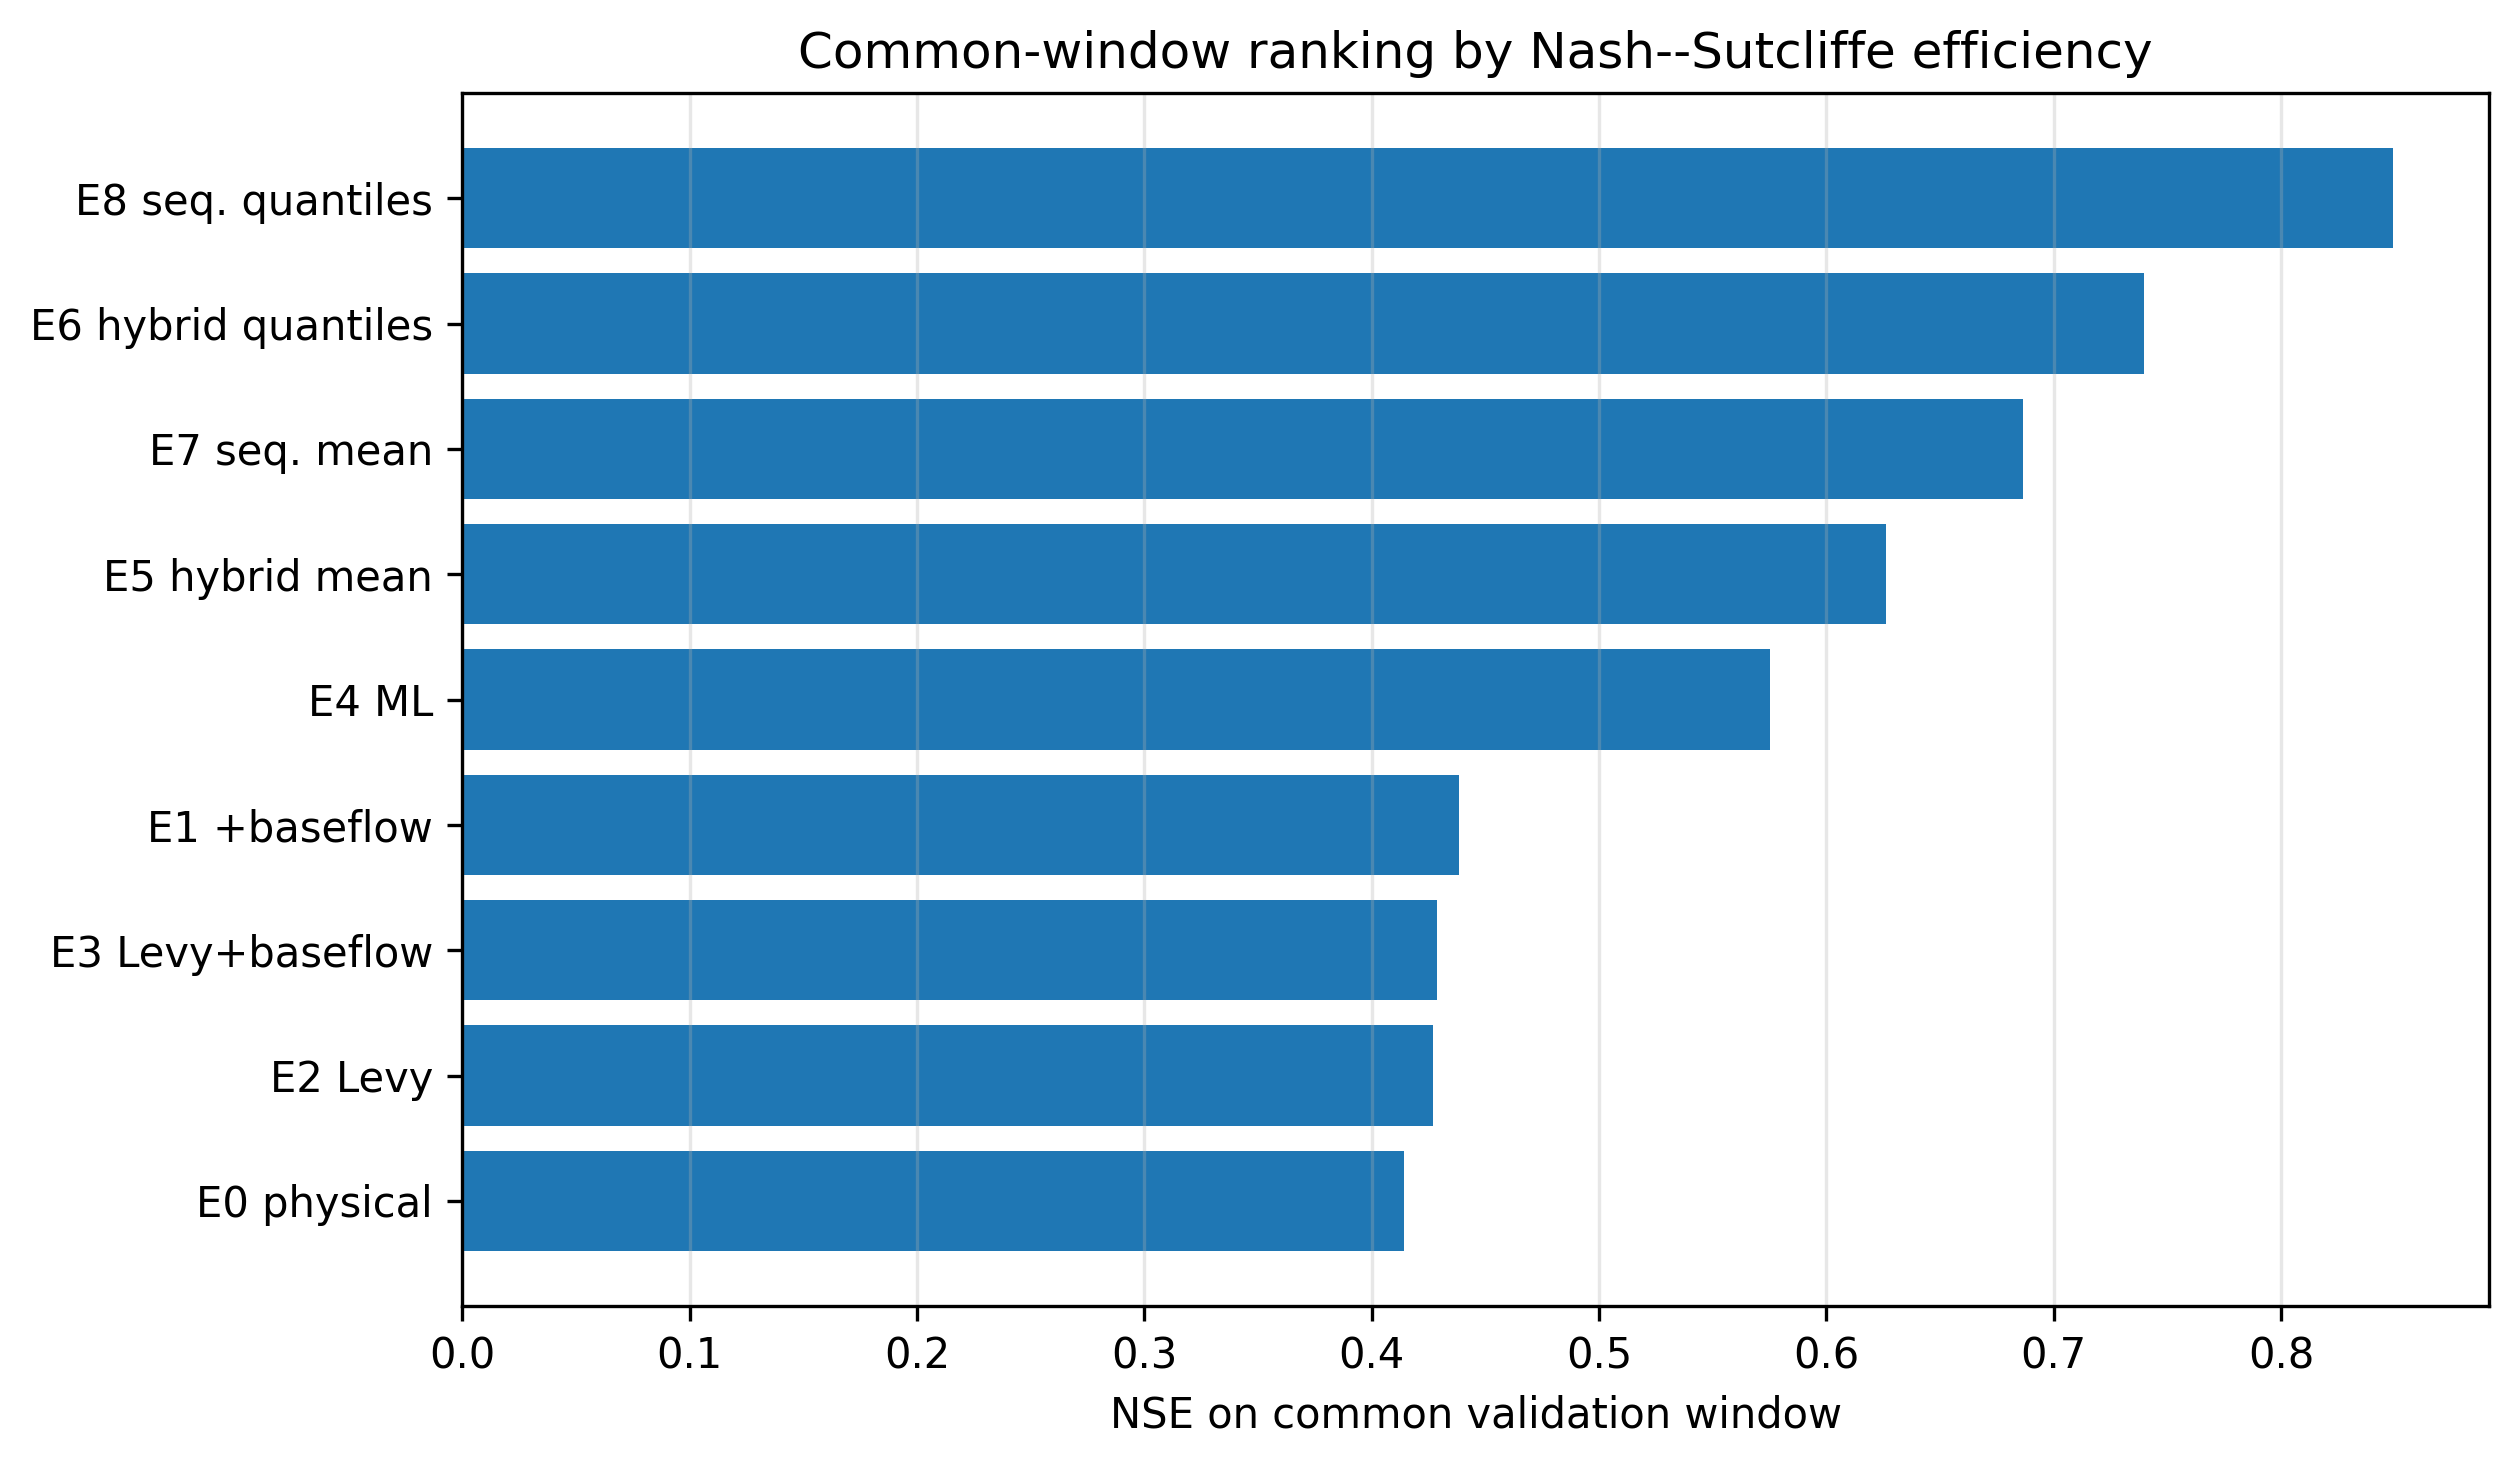
\includegraphics[width=0.95\linewidth]{figures/metric_ranking_nse.png}
\caption{Ranking of all experiments by common-window NSE. Numerical
values correspond to Table~\ref{tab:ranking}.}
\label{fig:metric-ranking}
\end{figure}

\subsection{Hydrograph and flow-duration behaviour}
\label{subsec:hydro-results}

The validation hydrograph in Fig.~\ref{fig:hydrograph-common} shows
that the hybrid models reproduce the timing and amplitude of seasonal
streamflow fluctuations more closely than the physical-only baselines.
The physical models retain the main wet-season response but frequently
collapse towards near-zero discharge during recession periods. This
behaviour is also evident in the flow-duration curves
(Fig.~\ref{fig:fdc-common}), where E0 shows an unrealistic decline in
the high-exceedance tail. Adding the baseflow reservoir reduces this
problem only partially, indicating that the single linear storage term
improves recession persistence but does not fully resolve dry-season
memory.

The hybrid configurations provide a closer match to the observed
flow-duration curve over most exceedance probabilities. The largest
visual improvement occurs in the lower-flow tail, where quantile-based
hybrids avoid the extreme collapse of the deterministic physical
trajectory. Nevertheless, the hydrograph also shows remaining errors
during sharp wet-season peaks. Thus, the hybrid improvement is not a
complete correction of event-scale dynamics; it is mainly a reduction
of systematic distributional errors and dry-season underestimation.

\begin{figure*}[t]
\centering
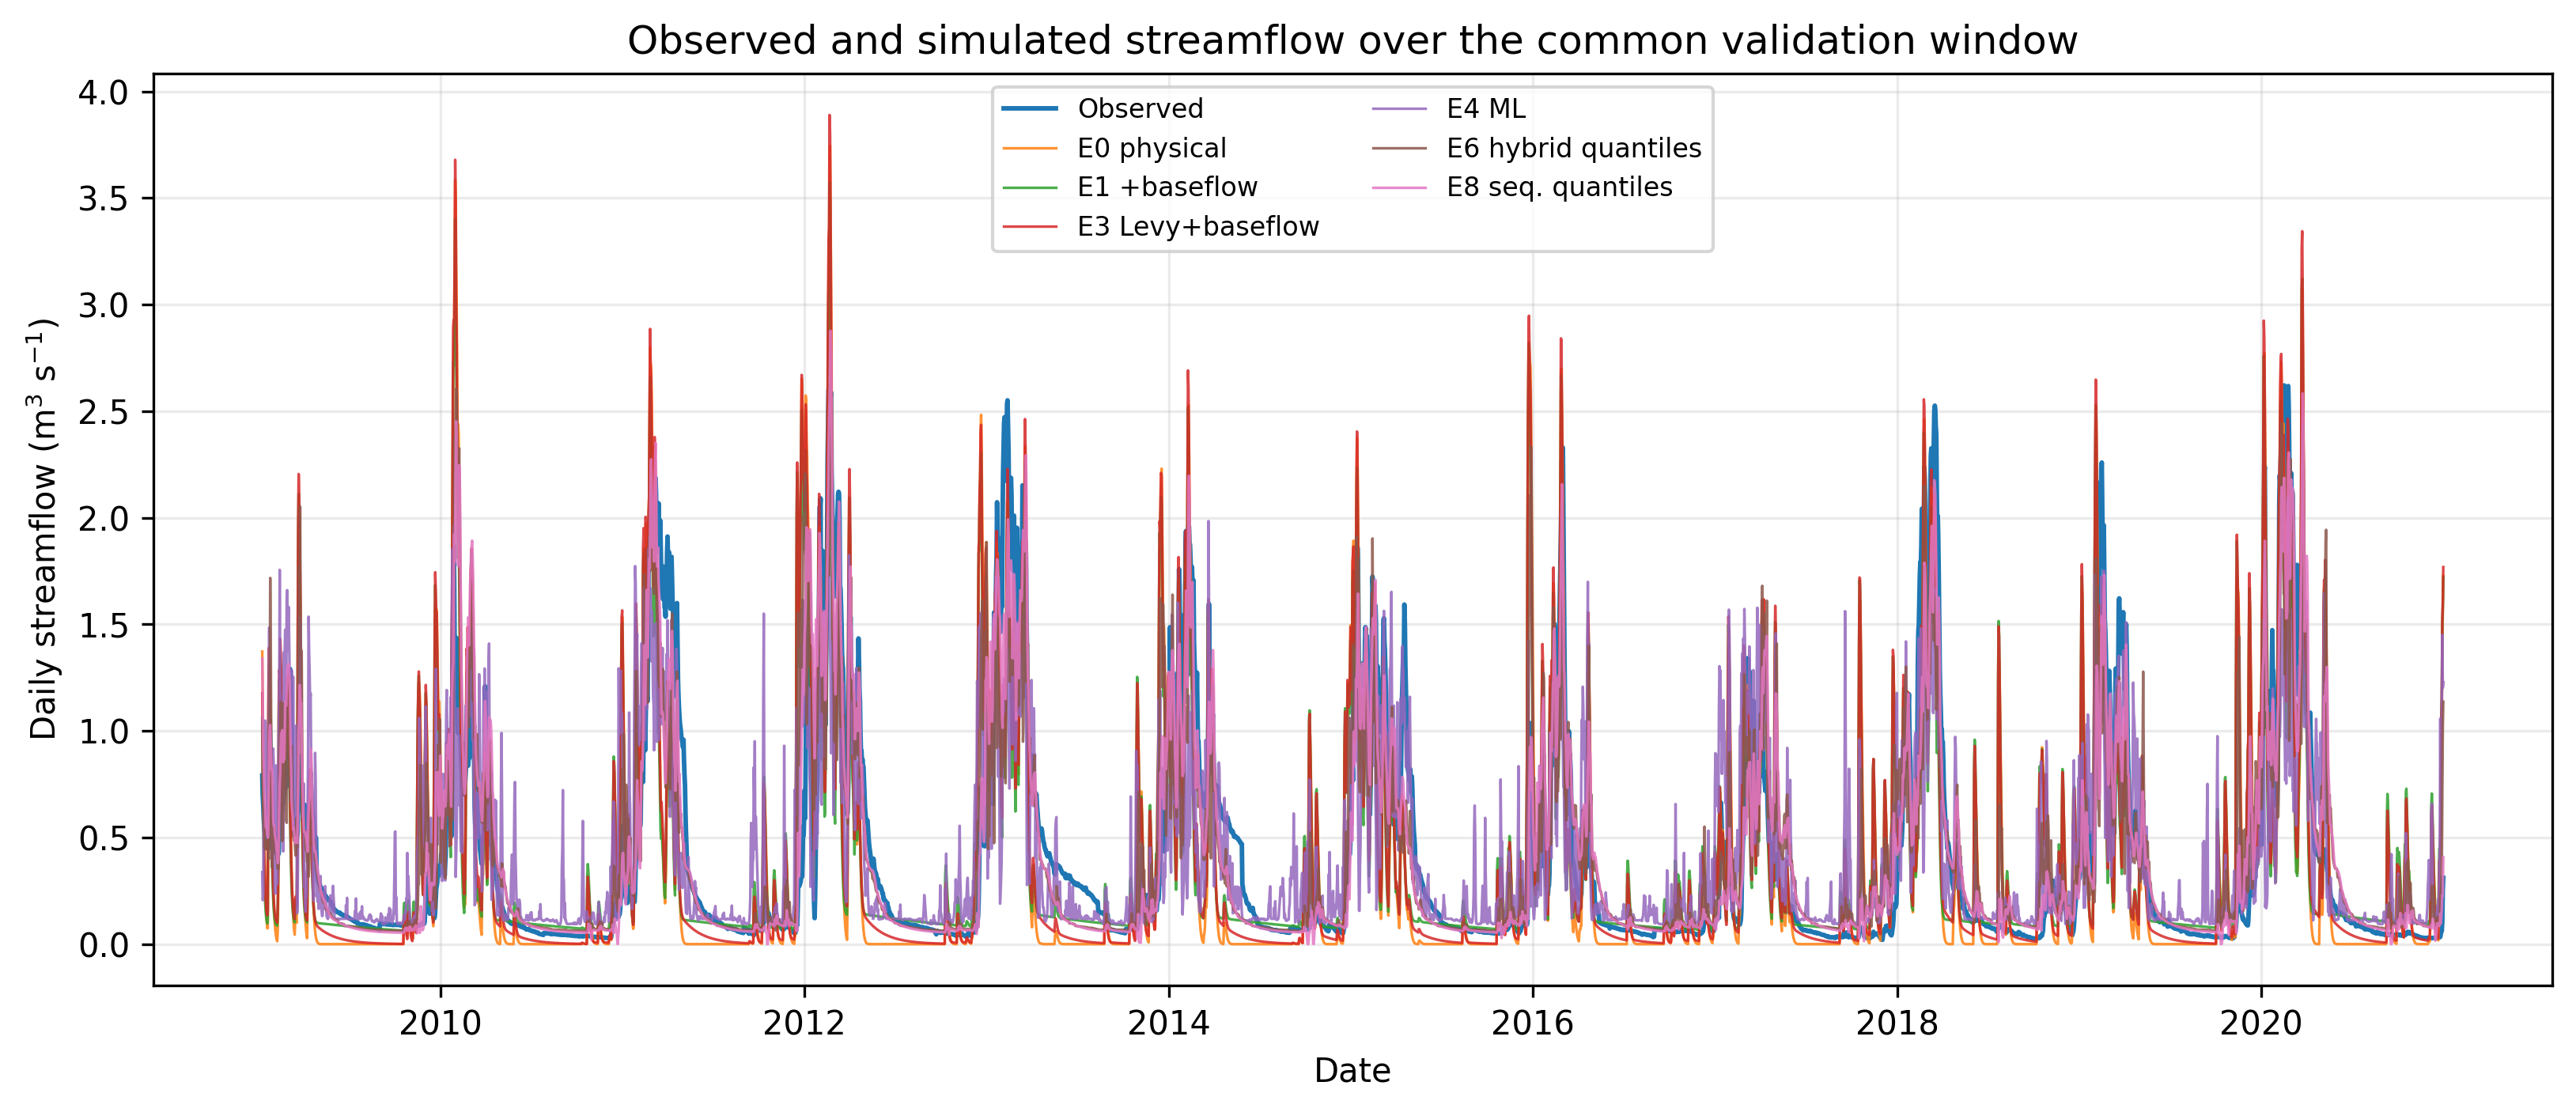
\includegraphics[width=0.98\textwidth]{figures/hydrograph_validation_common.png}
\caption{Observed and simulated daily discharge over the common
validation window for representative physical, pure ML and hybrid
models.}
\label{fig:hydrograph-common}
\end{figure*}

\begin{figure}[t]
\centering
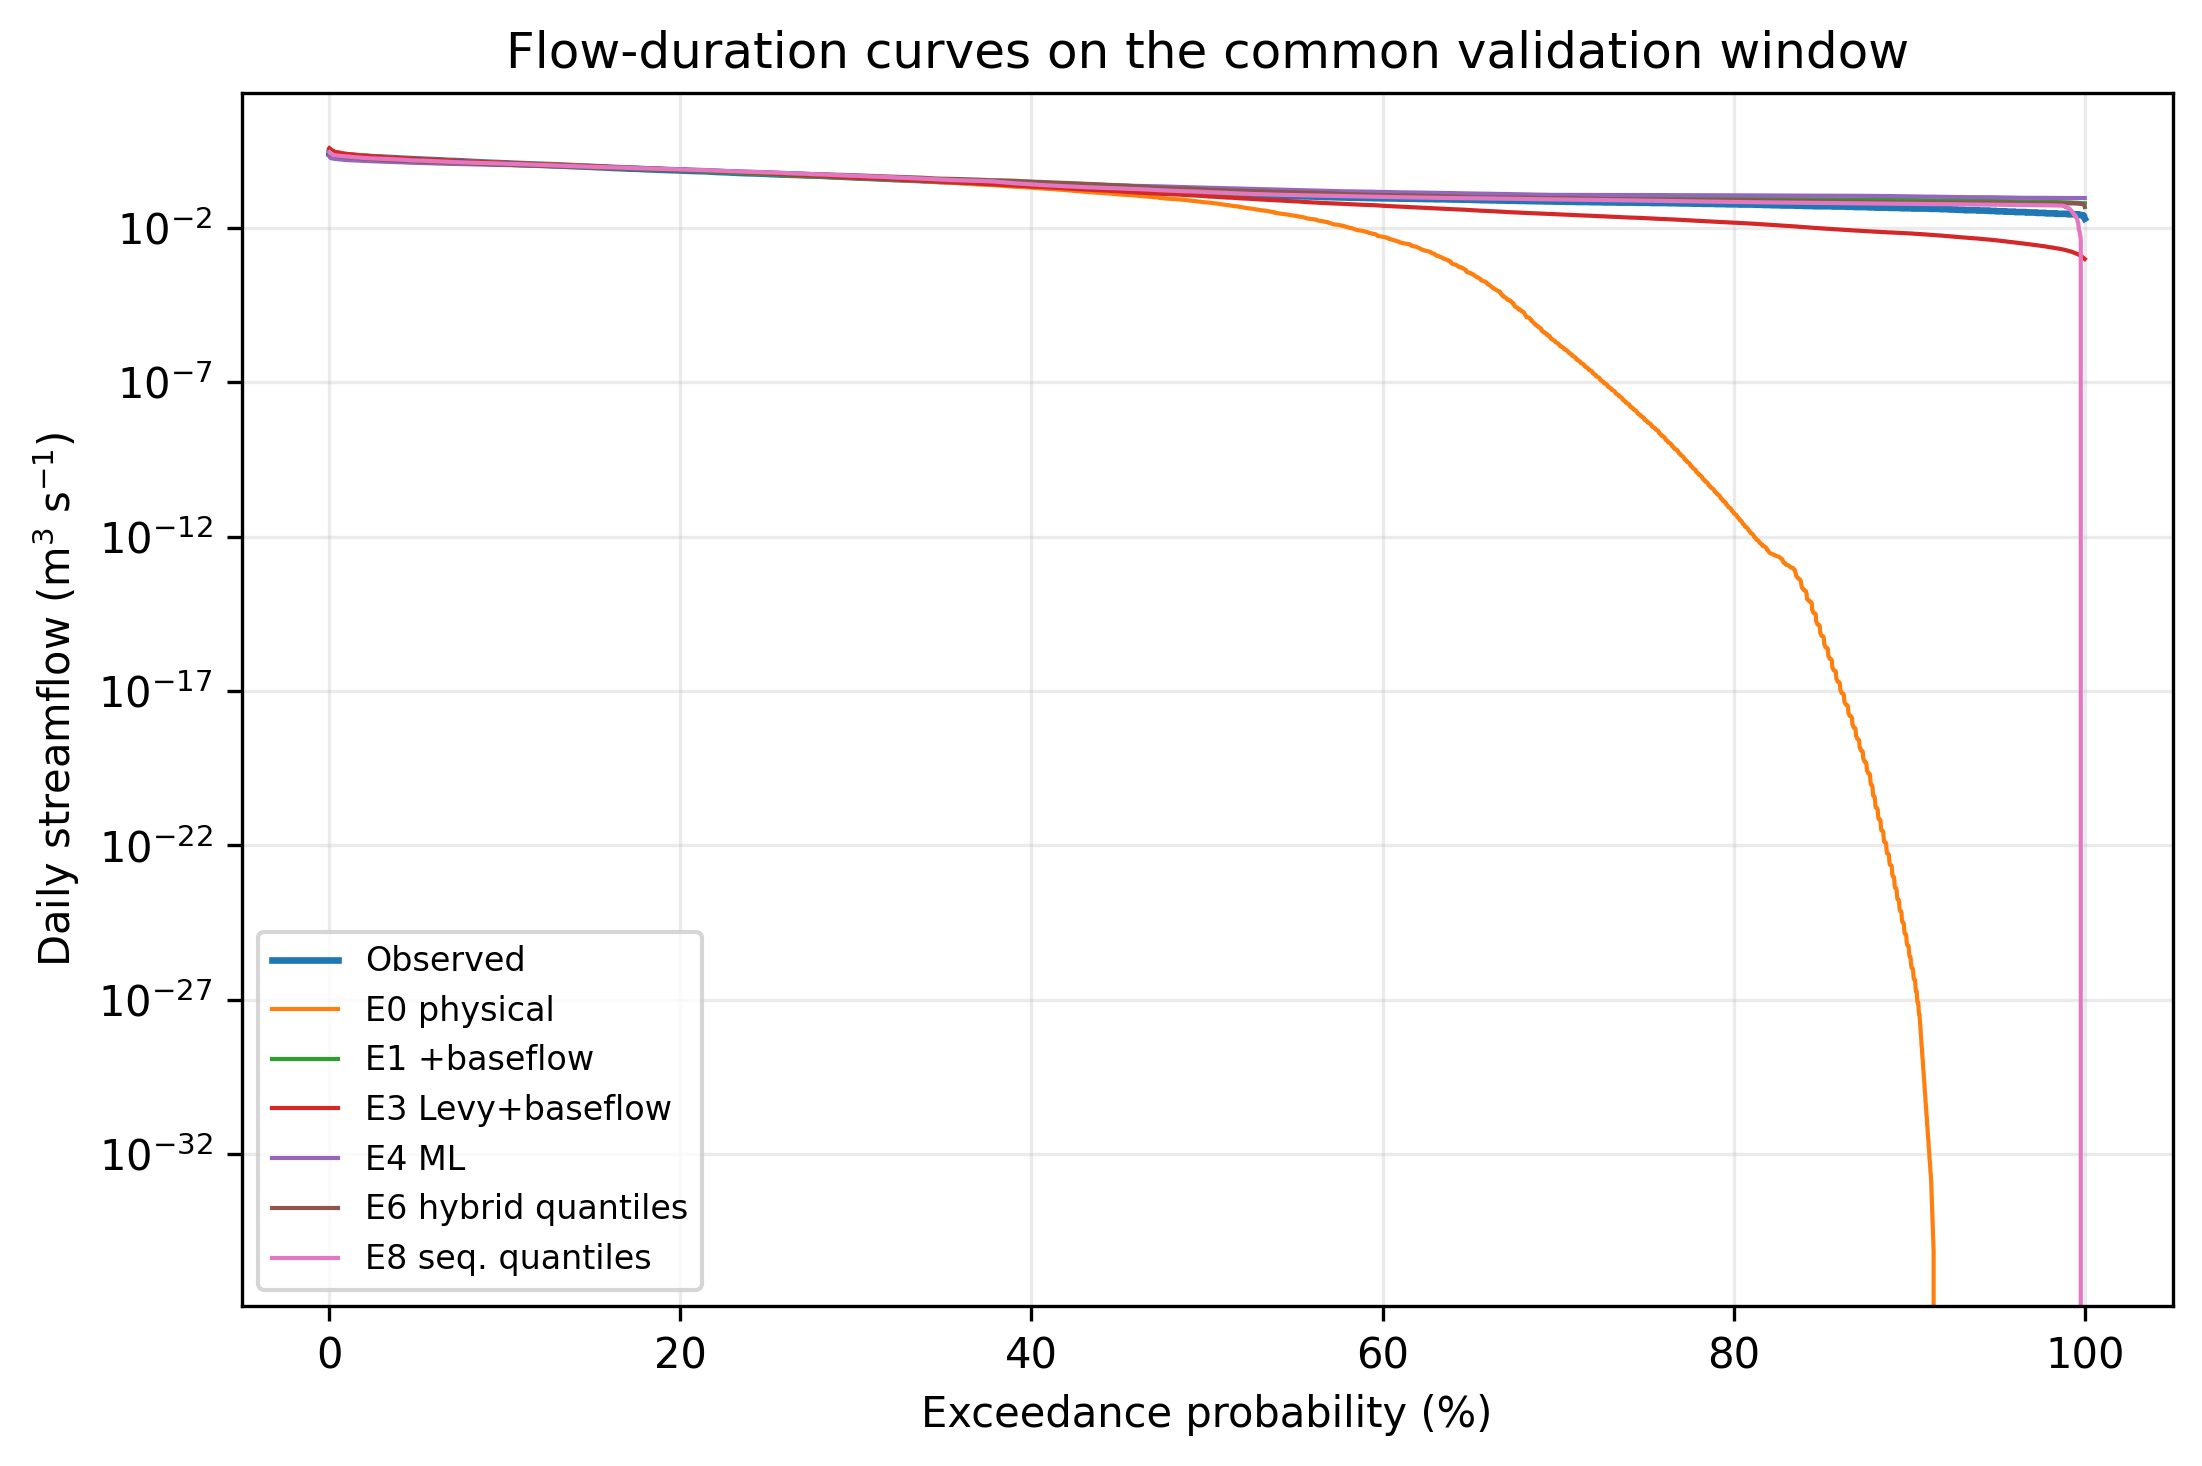
\includegraphics[width=0.95\linewidth]{figures/fdc_common.png}
\caption{Flow-duration curves for observed discharge and representative
simulations over the common validation window.}
\label{fig:fdc-common}
\end{figure}

\subsection{Ablation effects}\label{subsec:ablation-results}

Table~\ref{tab:ablation} and Fig.~\ref{fig:ablation-effects} isolate
the contribution of each modelling component. Adding the baseflow
reservoir to the deterministic physical model increased NSE by 0.024
and reduced RMSE by 0.009~m$^3$\,s$^{-1}$ (E1--E0). Under stochastic
forcing, the same structural addition produced a smaller but still
positive gain in NSE and KGE (E3--E2). In contrast, adding
L\'{e}vy-type perturbations to the baseflow-enabled physical model did
not improve point-prediction skill: NSE decreased by 0.010 and RMSE
increased by 0.004~m$^3$\,s$^{-1}$, although KGE increased slightly.
This confirms that stochastic perturbation is not, by itself, the main
source of point-prediction improvement.

The dominant gain came from hybridization. Relative to the complete
stochastic physical baseline (E3), the pure forcing-based ML model
(E4) improved NSE by 0.147, whereas the XGB-labelled hybrid using
ensemble means (E5) improved NSE by 0.198. The quantile-based hybrid
(E6) produced the largest backend-consistent ablation effect, with
$\Delta$NSE\,=\,0.311 and $\Delta$RMSE\,=\,-0.133~m$^3$\,s$^{-1}$
relative to E3. The direct comparison between E6 and E5 added
0.114 NSE and 0.095 KGE, showing that ensemble quantiles carry useful
predictive information that is lost when the stochastic physical
ensemble is compressed to its mean alone.

The GRU-labelled contrasts must be interpreted with the backend audit
in mind. E7 and E8 improved over their XGB-labelled counterparts, but
these gains cannot be attributed to recurrent-network memory because
both runs used a fallback MLP backend. They are therefore reported as
additional sequential-feature experiments under fallback execution, not
as evidence that GRU architecture is superior.

\begin{table*}[t]
\caption{Ablation effects on the common validation window. Positive
$\Delta$NSE and $\Delta$KGE indicate improvement; negative
$\Delta$RMSE and $\Delta$MAE indicate error reduction.}
\label{tab:ablation}
\centering
\small
\begin{tabular*}{\textwidth}{@{\extracolsep{\fill}}lllrrrr@{}}
\toprule
Ablation & Baseline & Candidate
  & $\Delta$NSE & $\Delta$KGE & $\Delta$RMSE & $\Delta$MAE \\
\midrule
deterministic\_baseflow
  & E0\_RAMIS\_DET\_NOBF & E1\_RAMIS\_DET\_BF
  & 0.024 & 0.000 & -0.009 & -0.022 \\
stochastic\_baseflow
  & E2\_RAMIS\_LEVY\_NOBF & E3\_RAMIS\_LEVY\_BF
  & 0.002 & 0.008 & -0.001 & -0.012 \\
levy\_given\_baseflow
  & E1\_RAMIS\_DET\_BF & E3\_RAMIS\_LEVY\_BF
  & -0.010 & 0.011 & 0.004 & 0.008 \\
pure\_ml\_vs\_physical
  & E3\_RAMIS\_LEVY\_BF & E4\_ML\_PURE\_XGB
  & 0.147 & -0.064 & -0.056 & -0.033 \\
hybrid\_mean\_vs\_physical
  & E3\_RAMIS\_LEVY\_BF & E5\_HYB\_XGB\_MEAN
  & 0.198 & -0.010 & -0.078 & -0.046 \\
hybrid\_quantiles\_vs\_physical
  & E3\_RAMIS\_LEVY\_BF & E6\_HYB\_XGB\_QUANTILES
  & 0.311 & 0.085 & -0.133 & -0.094 \\
quantiles\_vs\_mean\_xgb
  & E5\_HYB\_XGB\_MEAN & E6\_HYB\_XGB\_QUANTILES
  & 0.114 & 0.095 & -0.055 & -0.048 \\
gru\_mean\_vs\_xgb\_mean
  & E5\_HYB\_XGB\_MEAN & E7\_HYB\_GRU\_MEAN
  & 0.060 & 0.074 & -0.028 & -0.018 \\
gru\_quantiles\_vs\_xgb\_quantiles
  & E6\_HYB\_XGB\_QUANTILES & E8\_HYB\_GRU\_QUANTILES
  & 0.109 & 0.089 & -0.066 & -0.038 \\
\bottomrule
\end{tabular*}
\end{table*}

\begin{figure}[t]
\centering
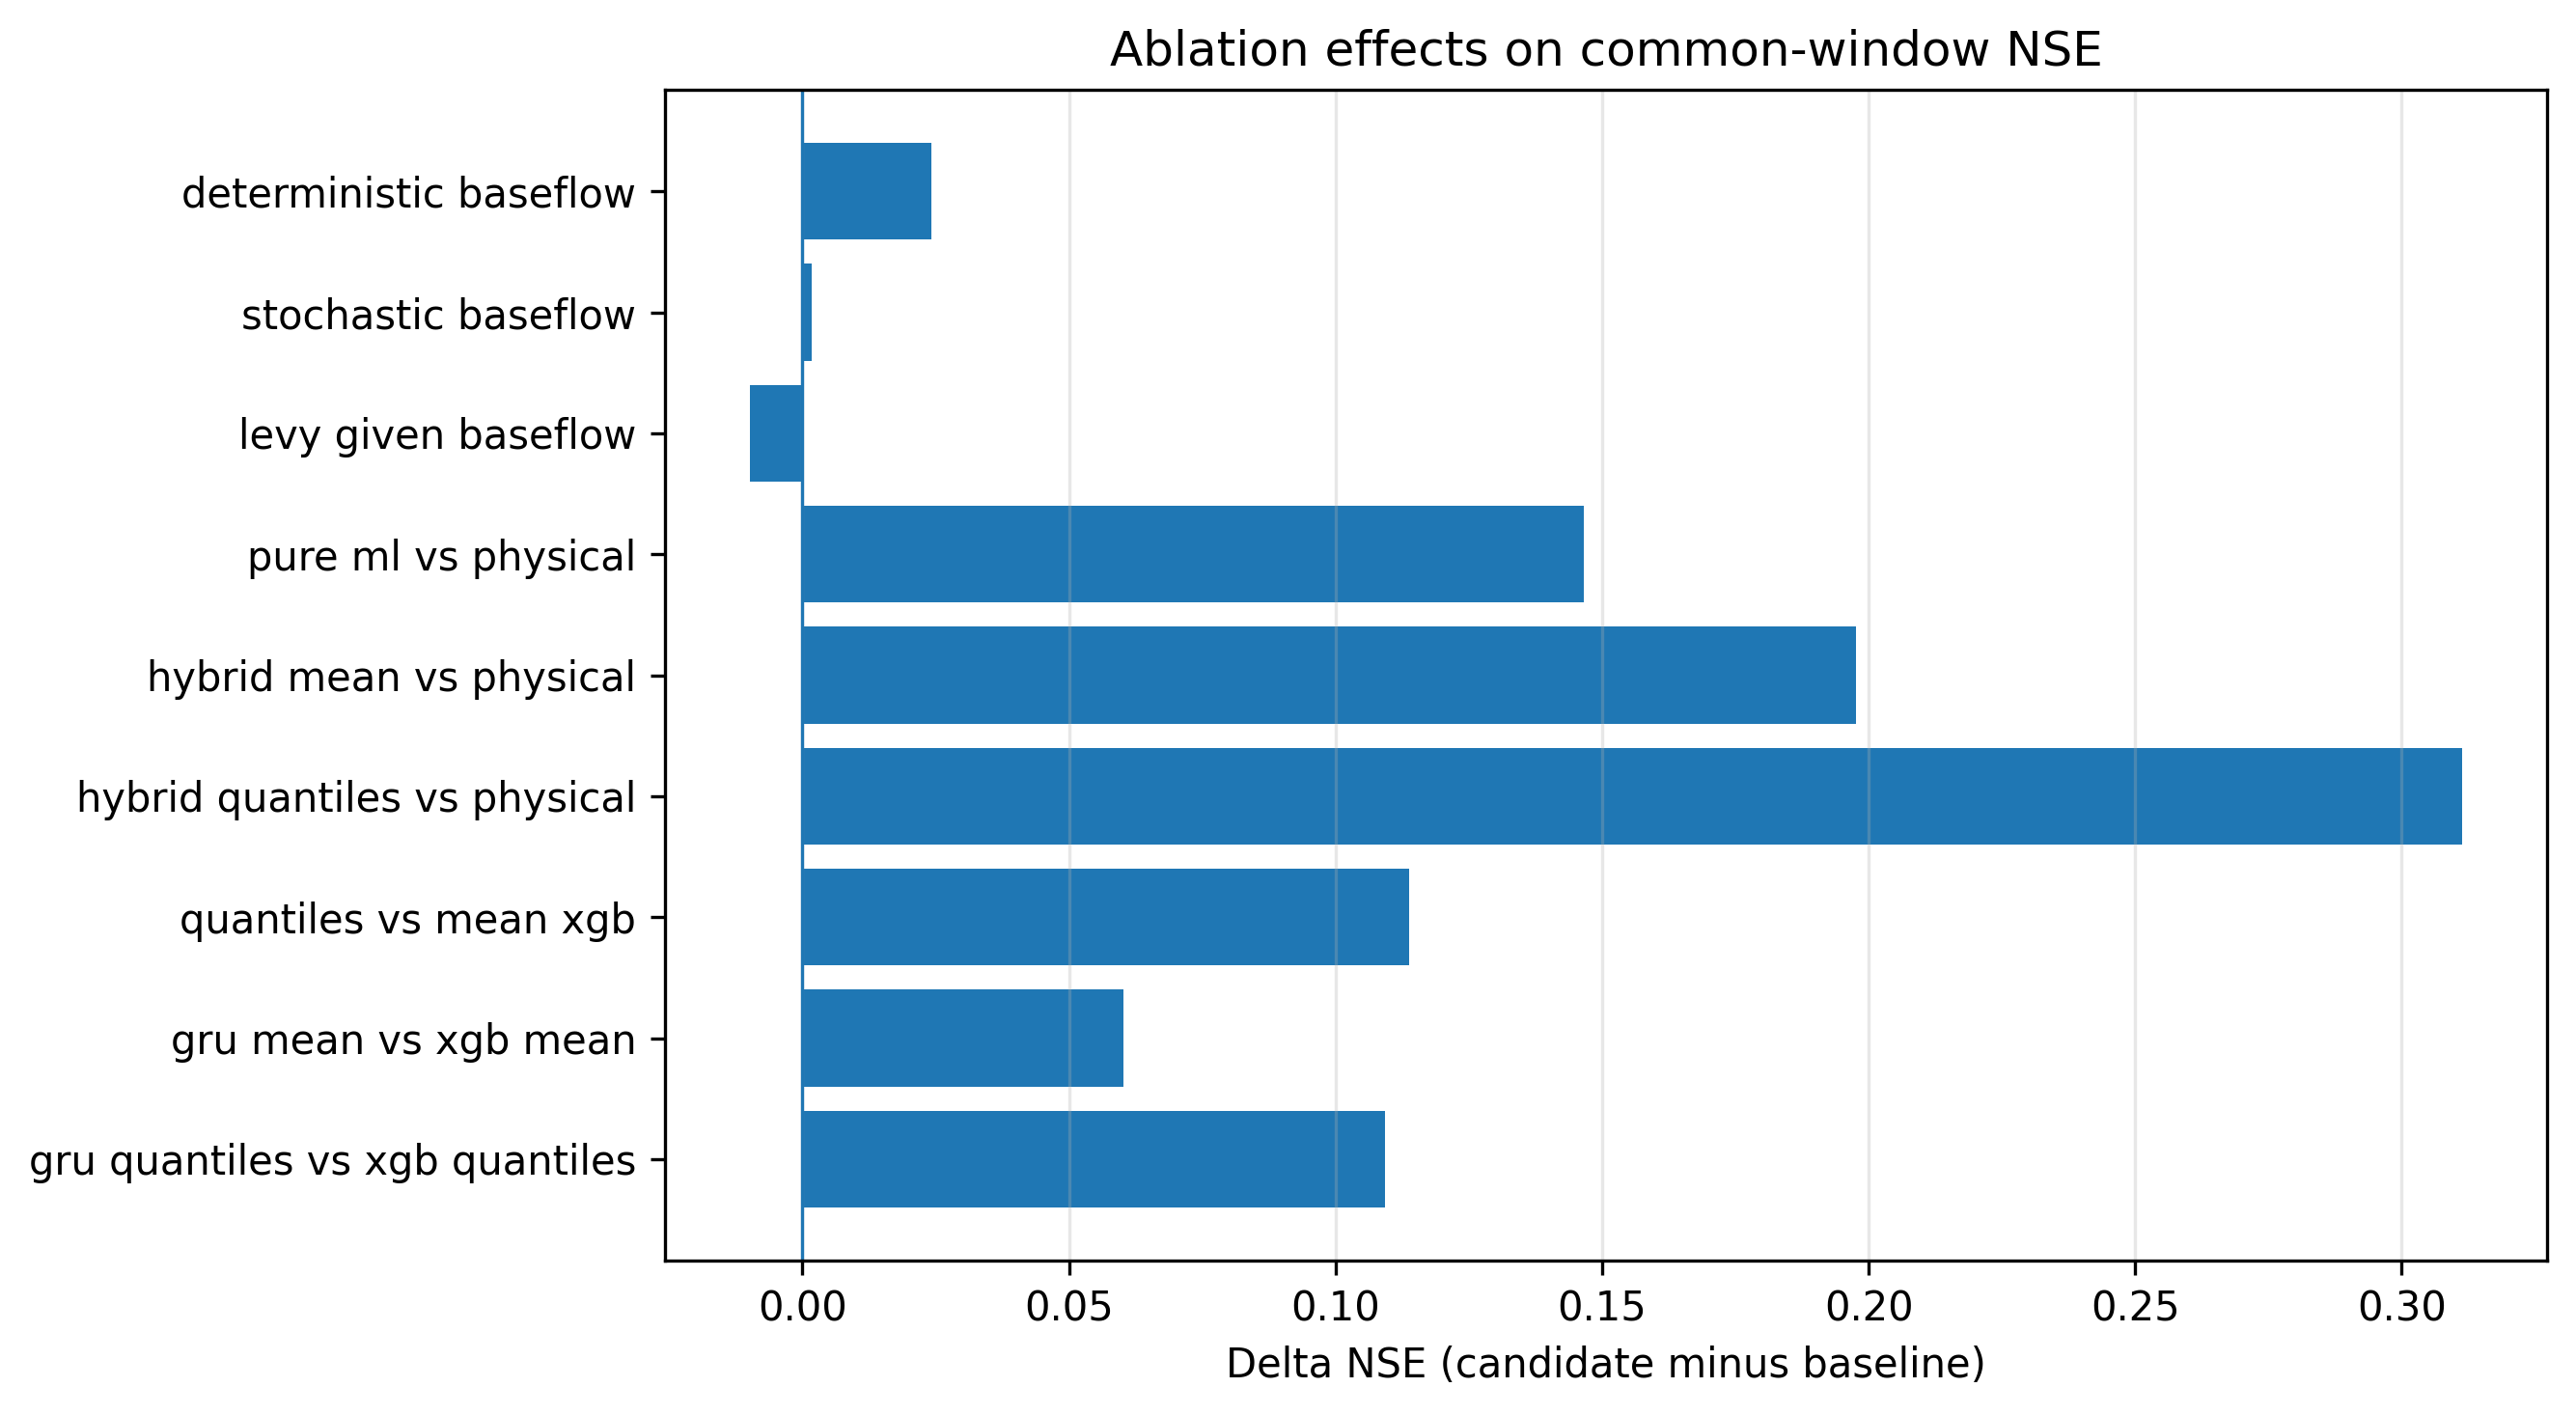
\includegraphics[width=0.95\linewidth]{figures/ablation_effects.png}
\caption{Ablation effects expressed as candidate-minus-baseline
$\Delta$NSE. Numerical values are reported in Table~\ref{tab:ablation}.}
\label{fig:ablation-effects}
\end{figure}

\subsection{Performance by flow regime}\label{subsec:regime-results}

Regime-specific RMSE values (Table~\ref{tab:regime-rmse} and
Fig.~\ref{fig:regime-rmse}) show that model skill is strongly
flow-dependent. The physical-only configurations had similar errors
across the selected regimes, with the largest absolute errors in the
high-flow class. The pure ML model reduced mid-flow RMSE relative to
the physical baselines, but its low-flow RMSE remained close to that of
the physical models. The quantile-based hybrid E6 substantially reduced
errors in all regimes, and the numerically best E8 configuration
further reduced RMSE under fallback-MLP execution.

The largest proportional improvement occurred in the low-flow regime:
RMSE decreased from 0.177~m$^3$\,s$^{-1}$ for E0 to
0.075~m$^3$\,s$^{-1}$ for E6 and 0.047~m$^3$\,s$^{-1}$ for E8. The
mid-flow and high-flow regimes also improved, but larger residual
errors persisted during high flows, where event timing and peak
magnitude remain more difficult to reproduce. These results support the
interpretation from the flow-duration curves: stochastic ensemble
quantiles are most useful for correcting systematic distributional
errors, especially during recession and low-flow periods, while peak
simulation remains only partially corrected.

\begin{table}[t]
\caption{RMSE (m$^3$\,s$^{-1}$) by flow regime for representative
models. Regime thresholds were estimated from calibration observations
only.}
\label{tab:regime-rmse}
\centering
\small
\begin{tabular*}{\linewidth}{@{\extracolsep{\fill}}lrrr@{}}
\toprule
Experiment & Low & Mid & High \\
\midrule
E0\_RAMIS\_DET\_NOBF   & 0.177 & 0.392 & 0.615 \\
E1\_RAMIS\_DET\_BF     & 0.197 & 0.365 & 0.613 \\
E3\_RAMIS\_LEVY\_BF    & 0.185 & 0.387 & 0.604 \\
E4\_ML\_PURE\_XGB      & 0.189 & 0.276 & 0.566 \\
E6\_HYB\_XGB\_QUANTILES & 0.075 & 0.222 & 0.461 \\
E8\_HYB\_GRU\_QUANTILES & 0.047 & 0.171 & 0.352 \\
\bottomrule
\end{tabular*}
\end{table}

\begin{figure}[t]
\centering
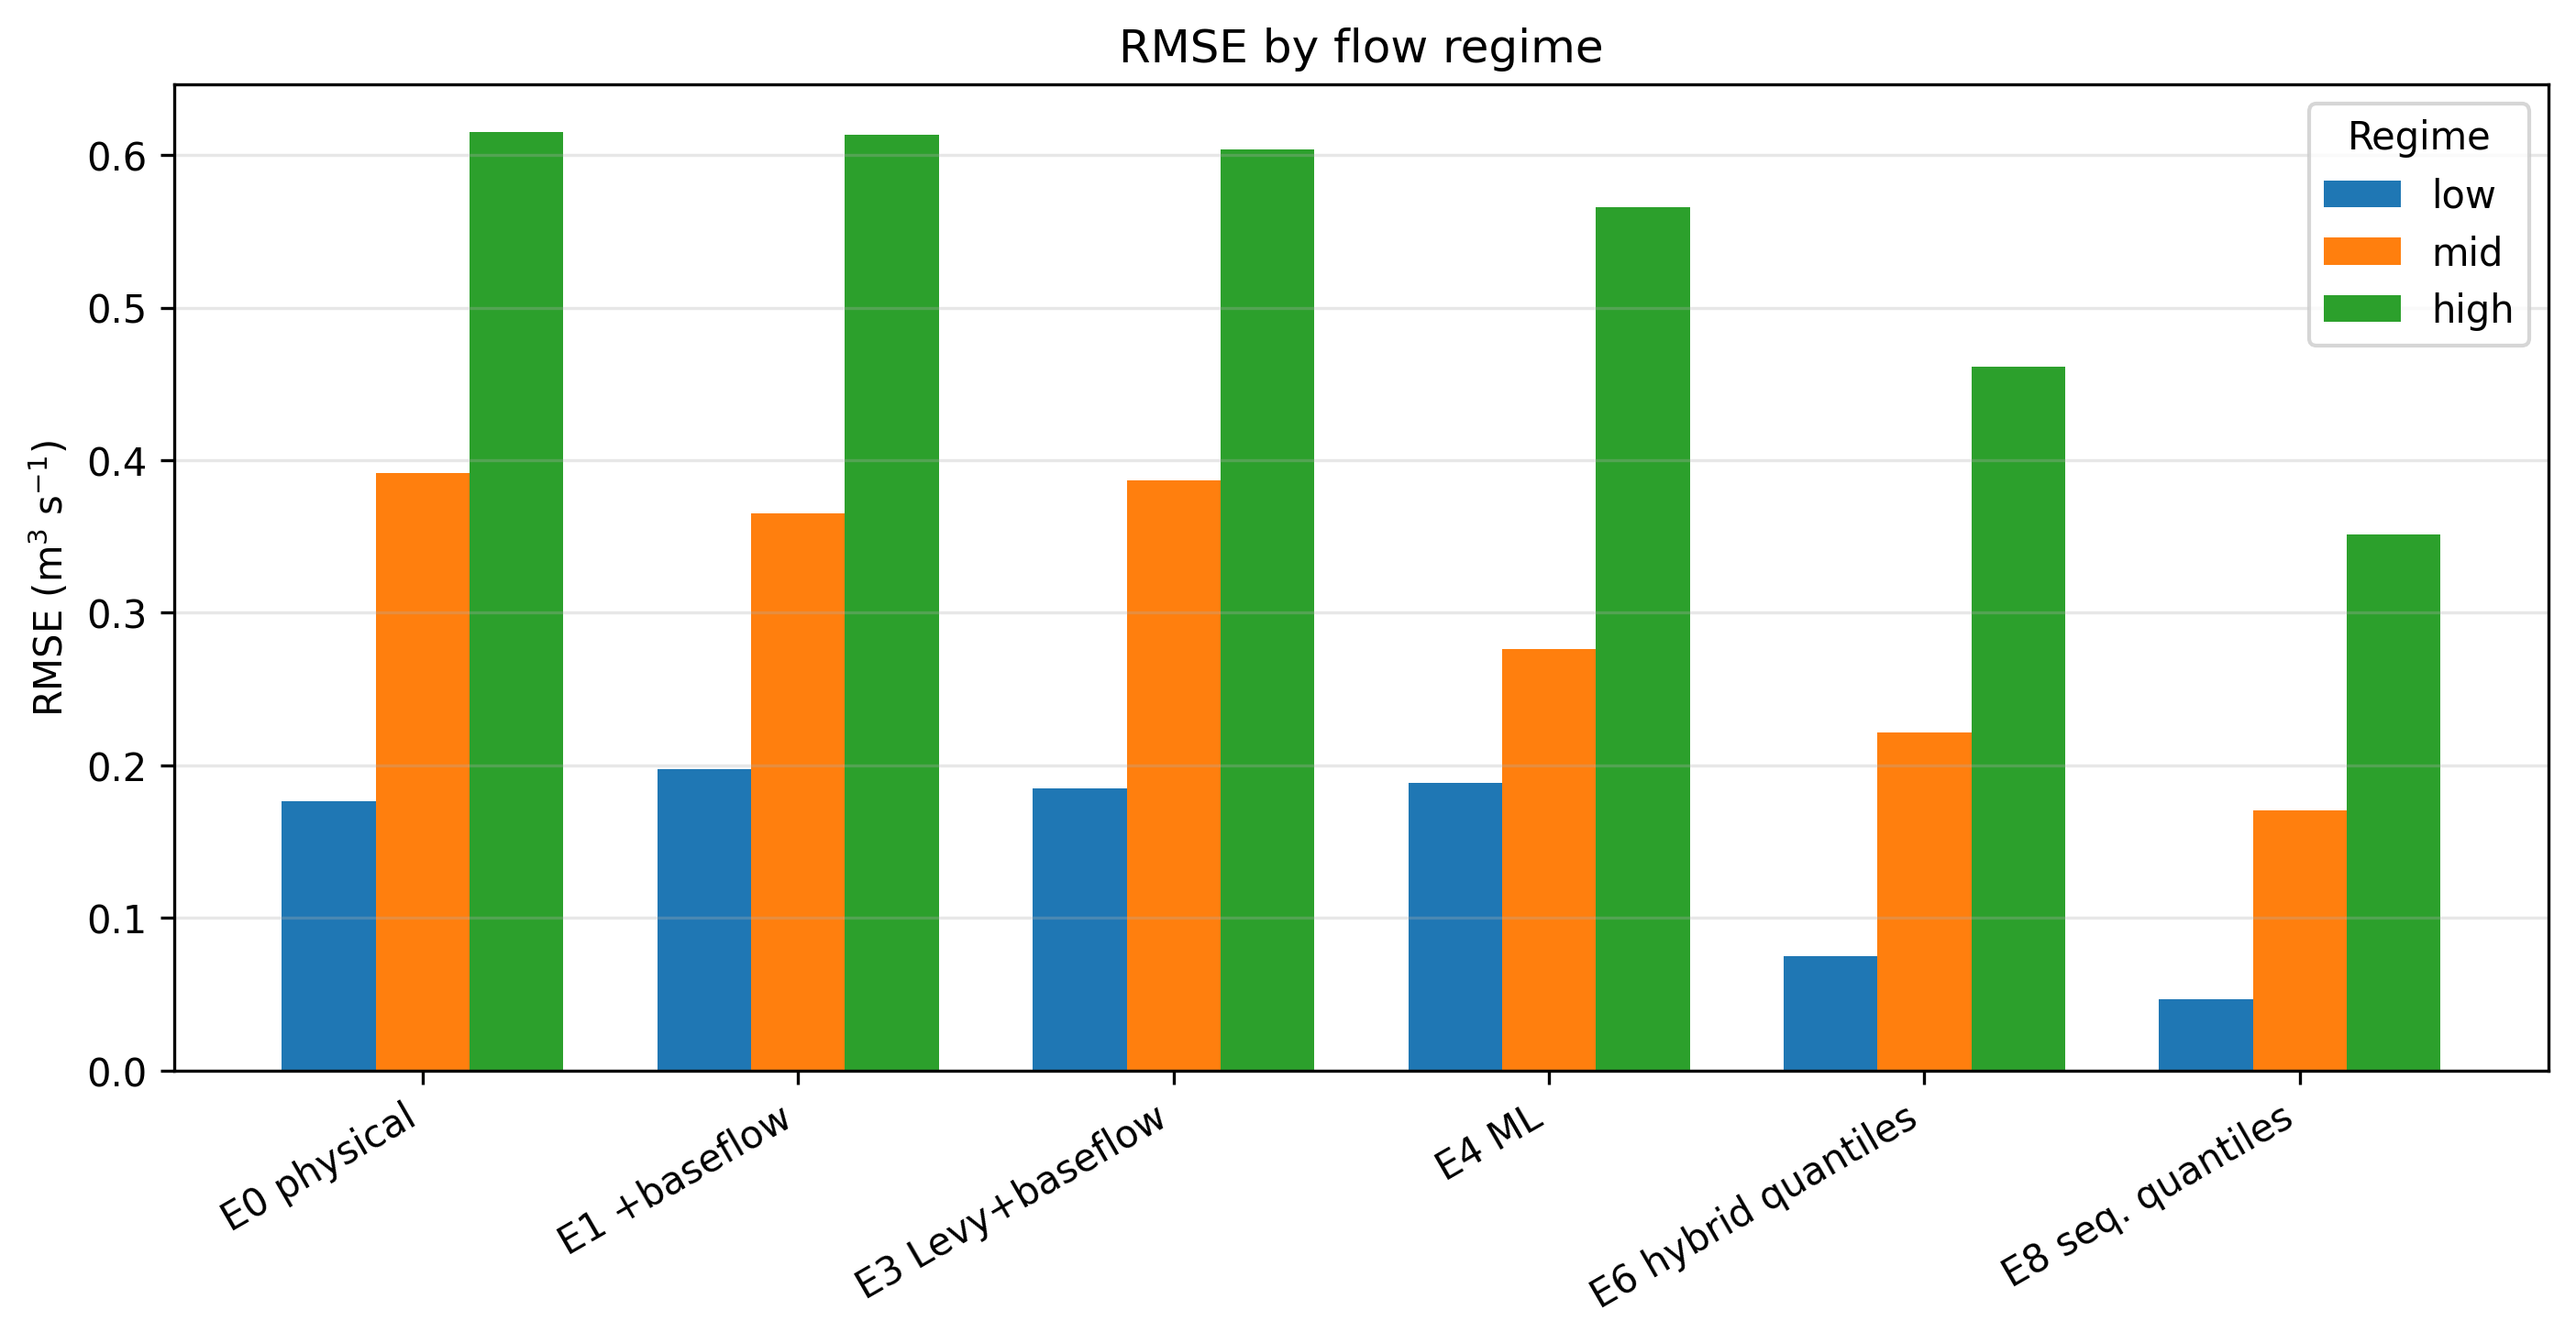
\includegraphics[width=0.95\linewidth]{figures/regime_rmse.png}
\caption{RMSE by low, mid and high flow regimes for representative
models. Values correspond to Table~\ref{tab:regime-rmse}.}
\label{fig:regime-rmse}
\end{figure}

\subsection{Uncertainty diagnostics and backend audit}
\label{subsec:uncertainty-results}

The stochastic physical intervals were strongly underdispersive
(Table~\ref{tab:uncertainty} and Fig.~\ref{fig:uncertainty-diagnostics}).
E2 achieved PICP\,=\,0.160 and E3 achieved PICP\,=\,0.004, both far
below the nominal 0.95 target. The corresponding PINAW values were also
small, particularly for E3 (PINAW\,=\,0.003), indicating that the
intervals were narrow rather than reliably calibrated. The high Winkler
scores confirm that most observed values fell outside the nominal
intervals. Consequently, the stochastic ensemble should not be reported
as a calibrated predictive uncertainty product in its current form. Its
main demonstrated value is as a source of physically structured
features for ML correction.

Table~\ref{tab:backend} summarizes the backend audit. The XGB-labelled
experiments (E4--E6) used the \texttt{sklearn\_hgb} backend, whereas
the GRU-labelled experiments (E7 and E8) used
\texttt{fallback\_mlp\_on\_flattened\_sequences}. This distinction
changes the interpretation of the leaderboard: E8 may be reported as
the best numerical experiment, but not as evidence for recurrent neural
networks. The reproducibility checklist in
Table~\ref{tab:reproducibility} returned no FAIL item. WARN items were
associated with missing observed-flow values, low-flow physical
limitations, optional figure entries and the fallback backend, rather
than with direct evidence of temporal leakage.

\begin{table}[t]
\caption{Uncertainty diagnostics for stochastic physical reference
bands.}
\label{tab:uncertainty}
\centering
\small
\begin{tabular*}{\linewidth}{@{\extracolsep{\fill}}lrrrr@{}}
\toprule
Experiment & PICP & PINAW & MPIW & Winkler \\
\midrule
E2\_RAMIS\_LEVY\_NOBF & 0.160 & 0.084 & 0.219 & 7.297 \\
E3\_RAMIS\_LEVY\_BF   & 0.004 & 0.003 & 0.009 & 10.050 \\
\bottomrule
\end{tabular*}
\end{table}

\begin{figure}[t]
\centering
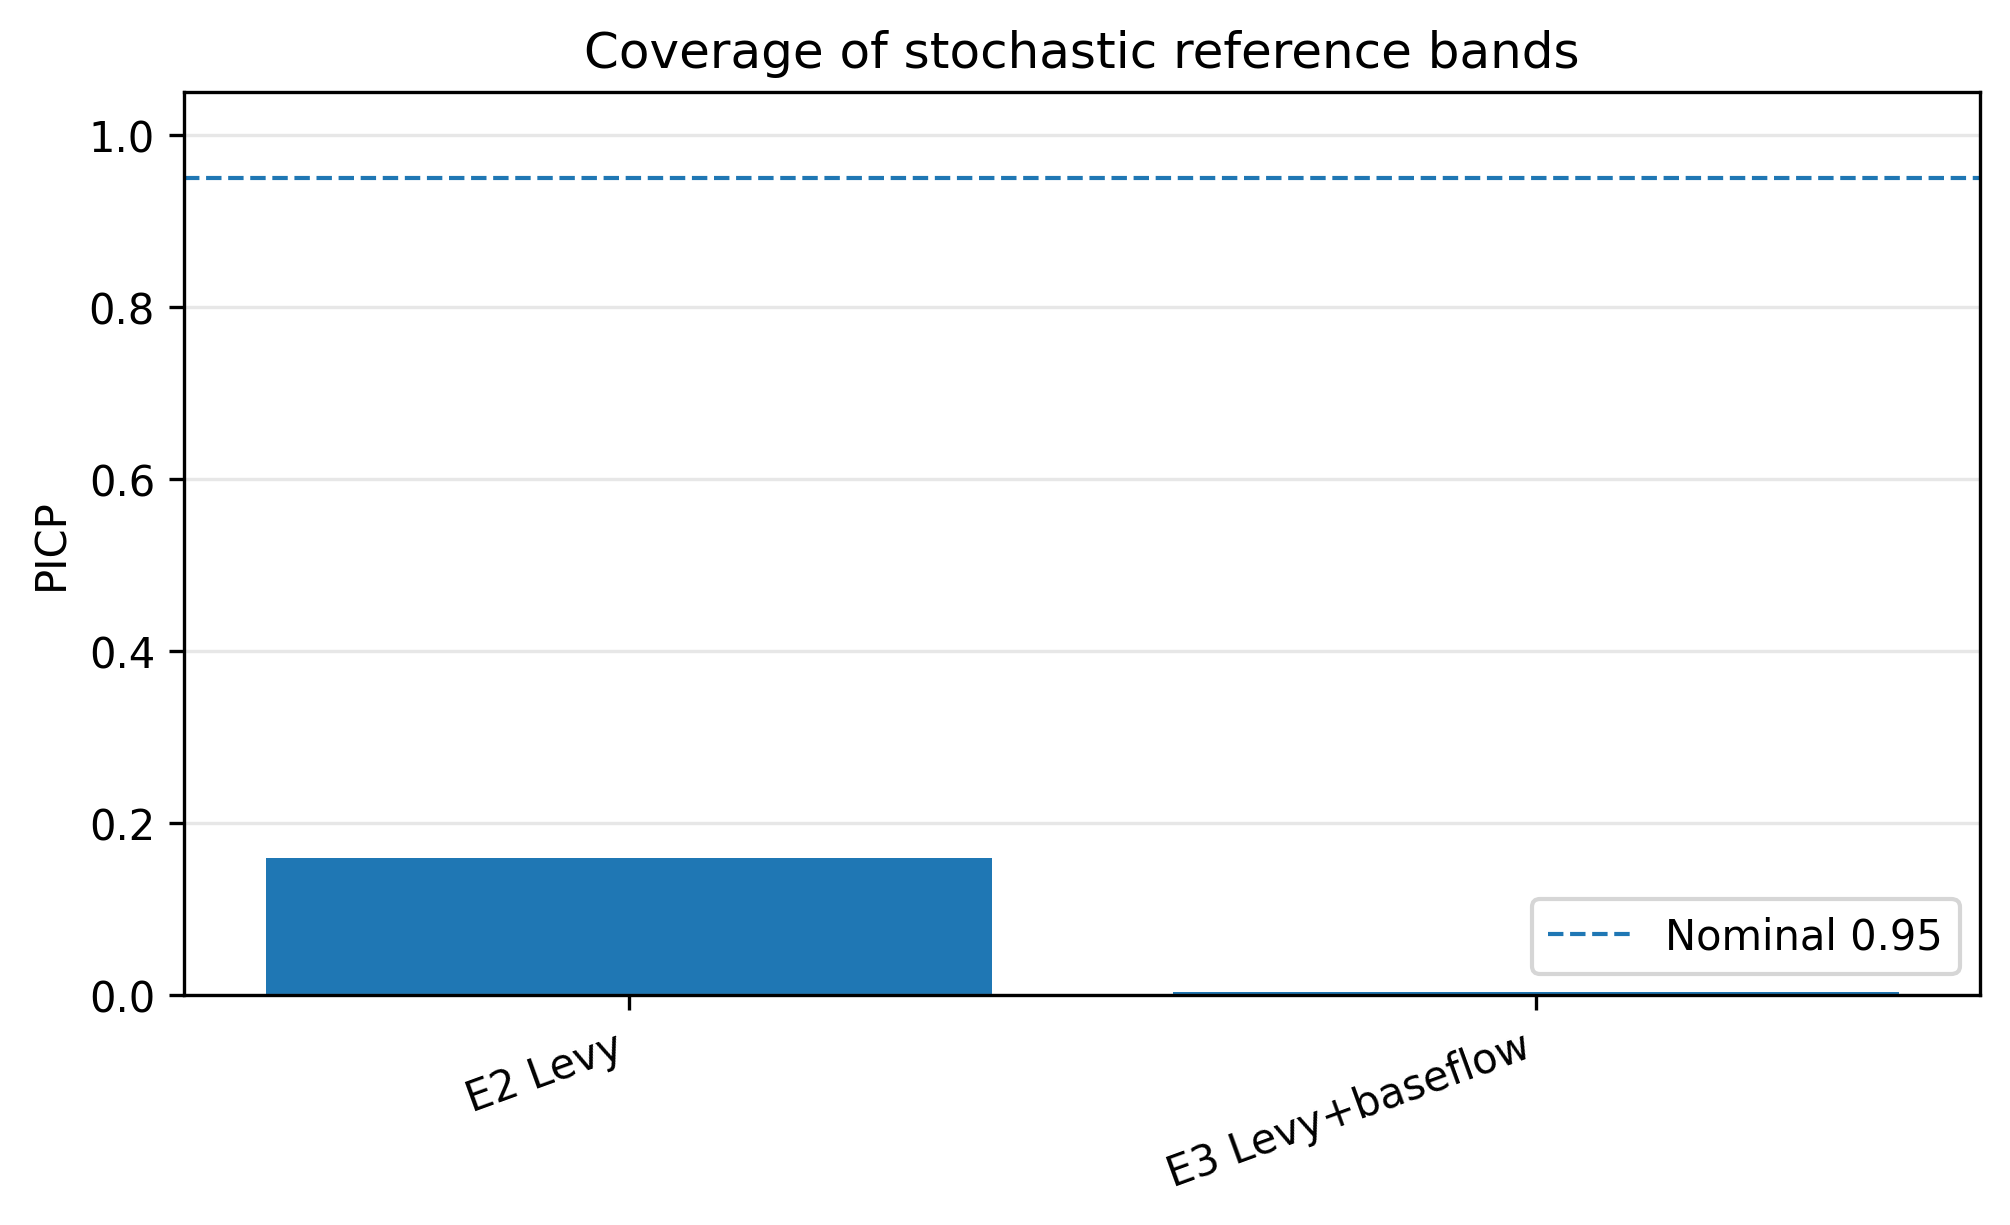
\includegraphics[width=0.95\linewidth]{figures/uncertainty_diagnostics.png}
\caption{Prediction interval coverage probability for stochastic
physical references. The dashed line marks the nominal 0.95 target.}
\label{fig:uncertainty-diagnostics}
\end{figure}

\begin{table*}[t]
\caption{Backend-aware manuscript notes for ML and hybrid configurations.}
\label{tab:backend}
\centering
\small
\begin{tabular*}{\textwidth}{@{\extracolsep{\fill}}p{0.22\textwidth}p{0.10\textwidth}p{0.24\textwidth}p{0.17\textwidth}p{0.20\textwidth}@{}}
\toprule
Experiment & ML label & Backend label & Feature source
  & Manuscript claim \\
\midrule
E4\_ML\_PURE\_XGB      & xgboost & sklearn\_hgb & observed\_forcing
  & report as gradient boosting (HGB) \\
E6\_HYB\_XGB\_QUANTILES & xgboost & sklearn\_hgb & stochastic\_ensemble
  & report as gradient boosting (HGB) \\
E7\_HYB\_GRU\_MEAN     & gru & fallback\_mlp\_on\_flattened\_sequences
  & stochastic\_ensemble & fallback MLP, not real recurrent GRU \\
E8\_HYB\_GRU\_QUANTILES & gru & fallback\_mlp\_on\_flattened\_sequences
  & stochastic\_ensemble & fallback MLP, not real recurrent GRU \\
\bottomrule
\end{tabular*}
\end{table*}

\begin{table*}[t]
\caption{Reproducibility checklist for the current evidence package.}
\label{tab:reproducibility}
\centering
\small
\begin{tabular*}{\textwidth}{@{\extracolsep{\fill}}lll@{}}
\toprule
Item & Status & Evidence \\
\midrule
Common validation intersection & PASS
  & leaderboard\_common\_intersection.csv \\
Anti-leakage audit & WARN & leakage\_audit\_status.txt=WARN \\
Physical audit   & WARN & physical\_audit\_status.txt=WARN \\
Figure manifest  & PASS
  & outputs/figures/phase34/phase34\_figure\_manifest.csv \\
GRU wording      & WARN & E7/E8 use fallback backend \\
Optional physical components in figures & WARN
  & skipped entries in phase34\_figure\_manifest.csv \\
\bottomrule
\end{tabular*}
\end{table*}


%% =====================================================================
%% 4. DISCUSSION
%% =====================================================================
\section{Discussion}\label{sec:discussion}

\subsection{Hydrological memory and the role of baseflow}
\label{subsec:discussion-baseflow}

The positive deterministic contrast E1--E0 confirms that adding a
linear baseflow reservoir improves the physical RAMIS baseline, in
agreement with the modelling evidence from semi-arid Andean catchments
reviewed by \citet{nauditt2017}: ``the best simulations could be
achieved with separate parameter sets for varying hydro-climatic
conditions,'' and a dedicated slow-drainage component is necessary to
represent the recession-dominated dry season. The NSE and RMSE
improvements are modest in absolute terms but hydrologically
meaningful: the baseflow reservoir introduces the delayed drainage
memory that cannot be captured by an instantaneous fast-flow response
alone. This conclusion echoes the quantitative demonstration of
\citet{adnan2021comparison} that including runoff memory in model
inputs is ``appropriate and contributes to an improvement of the models'
accuracy.''

However, the regime results in Table~\ref{tab:regime-rmse} show that
low-flow simulation remains challenging despite the presence of the
baseflow reservoir. A single linear store can represent average
recession behaviour but is insufficient when the storage is
heterogeneous across the catchment, as would be expected in an
Altiplano landscape with wetlands, peatlands (bofedales) and variable
permeability \citep{harman2009}. \citet{harman2009} showed
theoretically that ``between-hillslope heterogeneity alone can give
rise to apparently nonlinear recession slope curves,'' implying that
the effective storage--discharge relationship inferred from recession
analysis will always appear more complex than a simple linear
reservoir. A practical consequence for StoHyMoLAP is that the
baseflow improvement is bounded by the structural limitation of a
single-reservoir representation. This is consistent with the finding
of \citet{van2013} that ``parallel reservoirs with independent time
constants increase model performance in groundwater-dominated
catchments,'' suggesting a natural extension for future work.

The limited low-flow improvement also reflects a fundamental
measurement challenge: the NSE criterion assigns most weight to
high-flow variance \citep{pushpalatha2012}, so the global NSE
improvement from the baseflow reservoir is modest even when the
absolute error in the low-flow regime is reduced. Following the
recommendation of \citet{pushpalatha2012} to use the NSE on inverse
flows (NSE$^*_{iQ}$) to focus evaluation on the lowest 20\% of
flows, future studies should track this metric explicitly in addition
to global NSE.

\subsection{L\'{e}vy perturbations as stochastic descriptors rather
than calibrated uncertainty}\label{subsec:discussion-levy}

L\'{e}vy perturbations modify the distributional behaviour of physical
simulations and, in principle, can represent the heavy-tailed
variability documented for Andean precipitation and streamflow. The
coverage diagnostics in Table~\ref{tab:uncertainty}, however,
demonstrate that the resulting stochastic bands are strongly
underdispersive: PICP values of 0.16 and 0.004 are far below the
nominal 0.95, and Winkler scores reflect large penalties for missing
observations. This failure to achieve calibrated coverage is not
unique to L\'{e}vy-driven models: \citet{thiboult2016} showed that
even sophisticated multi-model ensemble systems ``fail to maintain
the required dispersion throughout the entire forecast horizon,'' and
\citet{crochemore2016} found that correcting precipitation inputs
alone is ``obviously not enough to achieve streamflow forecast
reliability.'' The more general point is that calibrated uncertainty
requires explicitly accounting for all sources of error
simultaneously---not only stochastic forcing, but also parameter
uncertainty, structural uncertainty and initial-condition uncertainty
\citep{demirel2013,thiboult2016}.

The underdispersive nature of the bands does not negate the value of
L\'{e}vy perturbations within StoHyMoLAP; it merely redirects that
value. Rather than serving as calibrated intervals, the stochastic
ensemble summaries---particularly the quantile descriptors in
Eq.~\ref{eq:quantiles}---function as informative features that encode
distributional information about the conditional response of the
physical model. The key insight from \citet{gabellani2007} is directly
applicable here: ``the spectral slopes of the rain fields play an
essential role in determining the hydrological response,'' and features
that preserve asymmetry and tail behaviour (quantiles) carry more
information than features that collapse the distribution to its mean.
\citet{swiderski2016} showed that quantile representations are
``less sensitive to fat-tailed distributions and outliers,'' a
property that is particularly desirable when the ensemble members are
driven by $\alpha$-stable noise.

\subsection{Why quantile-based hybridization works}
\label{subsec:discussion-hybrid}

The most robust empirical signal in this study is the advantage of
quantile-based hybridization. The E6--E5 contrast adds 0.114 NSE and
0.095 KGE purely from switching the physical descriptor from a mean
to a quantile vector, holding everything else constant. This result
is interpretable within the framework of \citet{papacharalampous2022}:
``there are two ways for improving predictive performance---improving
the prediction algorithm and discovering new informative predictors,''
and quantile descriptors of the physical ensemble constitute precisely
the latter. A single ensemble mean retains first-moment information
but discards the conditional spread, asymmetry and tail behaviour of
the physical simulation. In the Ramis basin, where the flow regime
alternates sharply between wet-season peaks and dry-season recession,
these distributional properties are not constant: the upper quantiles
expand during the wet season while the lower quantiles collapse. This
asymmetric dynamics is informationally invisible to a mean-only
descriptor and yet is directly observable in the quantile vector.

The hybrid emulator (E6) also outperforms the pure ML baseline (E4)
despite E4 having access to observed meteorological forcing. This
indicates that physically simulated ensemble descriptors provide
information beyond what is contained in the observed forcings alone, a
result consistent with \citet{yang2020} who found NSE improvements of
23\% when ML surrogates were enriched with synthetic physical data, and
with \citet{mekonnen2015} who showed that SWAT outputs ``provide a
proxy about the instantaneous wetness condition of the catchment.''
The interpretation is that the physical ensemble descriptors
effectively encode catchment antecedent state in a form that the ML
emulator can more readily exploit than raw meteorological time series.
This is consistent with the argument of \citet{moreido2021} that ``a
machine learning model needs a teacher (hydrologist) that provides it
with textbooks and then leaves it for self-teaching,'' and with the
finding of \citet{okkan2021} that models lacking antecedent runoff
information cannot compete with physically constrained alternatives.

One should note, however, that the E6 advantage over E4 is partly
confounded with the difference in feature type (ensemble statistics
versus raw forcing), and the E6--E4 contrast alone cannot distinguish
between the value of hydrological structure and the value of temporal
aggregation. Resolving this would require an additional ablation
experiment pairing observed forcing with quantile features derived from
simple lag statistics, which is left for future work. This caveat is
consistent with the general warning of \citet{zhong2023} that
``implicit coupling... requires more elaborate design of the model
structure and inputs, as well as more thorough verification of the
results to avoid learning other misleading relationships.''

\subsection{Backend-aware interpretation of the sequential experiments}
\label{subsec:discussion-backend}

E8 is the top-ranked configuration in Table~\ref{tab:ranking}, but the
result must be interpreted together with Table~\ref{tab:backend}. The
fallback MLP backend in E7 and E8 processes flattened sequences rather
than recurrent hidden states, and therefore does not implement the
temporal gating mechanism that is the defining feature of GRU cells
\citep{cho2014gru,kratzert2018}. The valid conclusion is narrower:
a GRU-labelled sequential hybrid using quantile descriptors and
implemented with a fallback flattened-sequence MLP achieved the best
validation metrics in the current environment. Whether a true recurrent
GRU would reproduce or exceed this performance cannot be established
from the current evidence package.

The consistent ordering of quantile over mean descriptors in both the
XGB-labelled (E6$>$E5) and the GRU-labelled (E8$>$E7) families
suggests that the descriptor choice is the driver of improvement rather
than the emulator architecture. This is an important practical
conclusion: it implies that the gain from quantile hybridization should
be architecture-agnostic, and therefore reproducible under a true GRU
backend. Future work should rerun E7 and E8 with TensorFlow or PyTorch
backends and compare the GRU-specific gain to the descriptor-specific
gain measured here. Transparent backend reporting is essential for such
comparison, as emphasized by \citet{hall2021}: ``open hydrologists
document all components of their data collection and analysis pipeline,
favoring open and non-proprietary technologies.''

\subsection{Leakage, reproducibility and submission readiness}
\label{subsec:discussion-leakage}

The audit status in Table~\ref{tab:reproducibility} strengthens the
comparison by documenting the major leakage controls: strict temporal
splitting, non-negative lags, sequence construction within temporal
subsets, train-only scalers and train-only regime thresholds.
``Only 1\% of hydrology papers were fully reproducible'' in a recent
large-scale survey \citep{hall2021}, and the StoHyMoLAP audit is an
explicit step toward closing that gap.

The WARN status should remain visible in the manuscript or
supplementary material. WARN does not indicate detected temporal
leakage, but it does identify issues that affect interpretation:
missing observed-flow values, physical low-flow limitations,
underdispersive stochastic bands and fallback ML backends. These are
honest disclosures consistent with the open-science principles
advocated by \citet{hall2021} and with the rigorous benchmarking
framework recommended by \citet{papacharalampous2022}.

%% =====================================================================
%% 5. LIMITATIONS
%% =====================================================================
\section{Limitations}\label{sec:limitations}

This study has five main limitations. First, the sequential experiments
labelled as GRU were not executed with a real recurrent backend, so
their results cannot support claims about recurrent neural networks
\citep{kratzert2018}. Second, the L\'{e}vy stochastic bands are
underdispersive and should not be treated as calibrated uncertainty
intervals; recalibration following the guidelines of \citet{thiboult2016}
and \citet{abaza2017} is required before these bands can be used
operationally. Third, low-flow bias remains substantial despite
improvements in absolute-error metrics; future work should apply
the inverse-flow NSE criterion of \citet{pushpalatha2012} to focus
calibration explicitly on the dry-season regime. Fourth, the audit
status is WARN rather than fully PASS, requiring transparent reporting
of missing observations and physical-audit warnings. Fifth, %% [FILL]
confirm data provenance and units (Section~\ref{subsec:study-area}):
if the current package corresponds to an illustrative or
reduced-computation run, or if the discharge series is normalized or
refers to a sub-catchment rather than the full Puente Ramis basin, the
final submission must regenerate the complete evidence package with the
definitive, traceable observed Ramis dataset (source, station, units)
and publication-level calibration settings.

%% =====================================================================
%% 6. CONCLUSIONS
%% =====================================================================
\section{Conclusions}\label{sec:conclusions}

StoHyMoLAP provides a reproducible, audit-controlled framework for
evaluating stochastic physical--machine-learning hybridization in daily
streamflow simulation, applied here to the high-Andean Ramis basin in
the Lake Titicaca system. Four main conclusions emerge from the
controlled ablation.

First, quantile descriptors from the stochastic physical ensemble are
the dominant driver of hybrid improvement: replacing the ensemble mean
with quantile features added 0.114 NSE (E6--E5), and the full
quantile hybrid surpassed the physical model by 0.311 NSE (E6--E3).
This confirms, in an Altiplano setting, the argument of
\citet{papacharalampous2022} and the quantitative demonstration of
\citet{houenafa2025} that distributional descriptors carry information
beyond a single trajectory.

Second, the baseflow reservoir improves the deterministic physical
baseline (E1--E0: $\Delta$NSE\,=\,0.024) by introducing slow-drainage
memory consistent with the groundwater-dominated response of the Ramis
system \citep{nauditt2017}, but a single linear reservoir is
insufficient to fully correct the low-flow bias documented by
\citet{pushpalatha2012} and \citet{van2013}.

Third, L\'{e}vy perturbations improve point prediction inconsistently
as a direct physical forcing (E3--E1: $\Delta$NSE\,=\,$-$0.010) but
contribute positively as generators of ensemble diversity whose
distributional summaries serve as informative ML features. The
stochastic bands are strongly underdispersive (PICP\,=\,0.004 for E3)
and cannot be used as calibrated predictive intervals without further
post-processing \citep{thiboult2016,crochemore2016}.

Fourth, the numerically top-ranked configuration (E8, NSE\,=\,0.849)
must be reported as a GRU-labelled fallback-MLP run rather than as
evidence of recurrent neural-network superiority \citep{hall2021}.
The descriptor ordering (quantile\,$>$\,mean) is nevertheless
consistent across both emulator families, supporting the conclusion
that the information value of distributional physical descriptors is
architecture-agnostic.

Future work should regenerate E7 and E8 with real recurrent backends,
recalibrate stochastic uncertainty toward nominal coverage, apply
inverse-flow NSE criteria to improve low-flow performance, and
evaluate the framework at full-resolution Ramis data before
transferring to neighbouring Altiplano catchments.

%% =====================================================================
%% CODE AND DATA AVAILABILITY
%% =====================================================================
\section*{Code and data availability}

The manuscript tables and figures are generated from the StoHyMoLAP
Phase~3.4B--3.5 result package. The scripts
\texttt{make\_method\_diagram.py} and \texttt{build\_paper\_assets.py}
reproduce all figures and CSV tables. Backend metadata should be
regenerated after any change to the ML environment. %% [FILL] add
repository URL/DOI and the SENAMHI/ANA data-source citation.

\section*{Declaration of generative AI and AI-assisted technologies
in the writing process}

During preparation of this draft, AI-assisted writing was used to
organize the manuscript, convert reproducible artefacts into narrative
text, and generate supporting LaTeX scripts. The authors remain
responsible for verifying all scientific claims, numerical values,
references, data provenance and final wording before submission.

\section*{CRediT authorship contribution statement}

Jose Zevallos: Conceptualization of this study, Methodology, Software,
Writing -- original draft.

\section*{Declaration of competing interest}

The authors declare that they have no known competing financial
interests or personal relationships that could have appeared to
influence the work reported in this paper.

\section*{Acknowledgements}

%% [FILL] Acknowledgements, funding information and data-provider
%% credits (SENAMHI-Peru, ANA).
% To print the credit authorship contribution details (optional)
\printcredits


% Loading bibliography database
%% =====================================================================
%% BIBLIOGRAPHY
%% =====================================================================
\bibliographystyle{agsm}
\bibliography{ref}

\end{document}